\documentclass[fleqn, article, a4paper]{memoir}

% Swedish.
% \usepackage[T1]{fontenc}
% \usepackage[utf8]{inputenc}
% \usepackage[swedish]{babel}
\usepackage{pdfpages}

\usepackage[shortlabels]{enumitem}
\usepackage{selthcsexercise}
\usepackage{microtype}

% Utilities.
\usepackage{graphicx}
\usepackage[hyphens]{url}
\usepackage[swedish]{varioref}
\usepackage{listings}
\usepackage{fontspec} % To enable use of ttf fonts
\usepackage{enumitem} % For customizing lists

\usepackage{amsmath}  % For \text{}
\usepackage{pifont}   % Provides the star symbols
\usepackage[swedish]{babel}
\usepackage[autostyle, swedish=quotes]{csquotes}

%---------------------------------------------------------------

% Define the command for difficulty rating
\newcommand{\difficulty}[2][]{%
  \emph{Svårighet:} %
  \ifnum#2>0 \ding{72}\else \ding{73}\fi
  \ifnum#2>1 \ding{72}\else \ding{73}\fi
  \ifnum#2>2 \ding{72}\else \ding{73}\fi
  \ifnum#2>3 \ding{72}\else \ding{73}\fi
  \ifnum#2>4 \ding{72}\else \ding{73}\fi
  \ifx\relax#1\relax \else \hspace{3mm}(\textit{#1})\fi
  \par\noindent
}


% Set section count to -1, so the first section (which is hidden) becomes 0,
% and thus the first section actually becomes 1
\setcounter{section}{-1}

%---------------------------------------------------------------
\newenvironment{Hemarbete}%
{\begin{Assignments}[H]}{\end{Assignments}}

\newenvironment{Kontrollfragor}%
{\begin{Assignments}[K]\tightlist}{\end{Assignments}}

\newenvironment{Datorarbete}%
{\begin{Assignments}[D]}{\end{Assignments}}

\newenvironment{DatorarbeteCont}%
{\begin{Assignments}[D]\setcounter{Ucount}{\theSavecount}}{\end{Assignments}}

\newenvironment{Extrauppgifter}%
{\begin{Assignments}[E]}{\end{Assignments}}

\newenvironment{Deluppgifter}%
{\begin{enumerate}[a)]\firmlist}{\end{enumerate}}

% \newcommand{\file}[1]{{\slshape\fontfamily{ppl}\selectfont #1}}
\newcommand{\file}[1]{\texttt{#1}}

\newcommand{\commandchar}[1]{\textsc{#1}}

\newcommand{\progname}{c3pu}
\newcommand{\progversion}{v1.0}
\newcommand{\progfilename}{\progname-\progversion.jar}

% Define the hint command
\newcommand{\hint}[2][]{\par\halfblankline\noindent\textbf{Ledtråd\ifx#1\empty\else\space#1\fi}: #2\par}

\lstset{
	escapeinside={(*@}{@*)},
}

\setlist[description]{
	style=multiline,
	align=right,
	itemsep=1mm,
	parsep=0mm,
	rightmargin=1cm,
}

% Section styles.
\setsecheadstyle{\huge\sffamily\bfseries\raggedright} 
\setsubsecheadstyle{\Large\sffamily\bfseries\raggedright} 
\setsubsubsecheadstyle{\normalsize\sffamily\bfseries\raggedright} 

\setsecnumformat{} % numrera inte laborationerna
\renewcommand{\thesection}{\arabic{section}} % för referenser till laborationerna
\renewcommand{\thefigure}{\arabic{figure}}

%*****************************************************************
\author{}
\begin{document}

\clearpage
\thispagestyle{empty} % Removes page number
\vspace*{30mm}
\begin{center}
	\sffamily
	\renewcommand{\baselinestretch}{1.1}
	\Huge\bfseries Datorlaborationer \\[5mm]
	EDAB05 \\[2mm]
	\LARGE\bfseries	Datorer och datoranvändning \\[7mm]
	\large Lunds universitet, LTH --- \the\year
\end{center}
\clearpage


%*****************************************************************
\courseinfo{Datorer och datoranvändning}{\the\year}
\maketitle
\thispagestyle{titlepage}
\vspace{-4cm}
\section*{Datorlaborationer, Datorer och datoranvändning}

Datorlaborationerna ger exempel på tillämpningar av det material som behandlas under kursen. Schema för laborationerna (tider och datorsalar) finns i kursprogrammet och på kurshemsidan. För laborationerna gäller följande:

\begin{itemize}
	\item Laborationerna är obligatoriska. Det betyder att du måste bli godkänd på alla uppgifterna under ordinarie laborationstid. Om du skulle vara sjuk vid något laborationstillfälle så måste du anmäla detta till kursansvarig (\url{mattias.nordahl@cs.lth.se}) före laborationen. Om du varit sjuk bör du göra uppgiften på egen hand och redovisa den under ditt nästa laborationstillfälle. Det kommer också att anordnas en uppsamlingslaboration efter kursens slut, för de studenter som missat någon laboration.

	\item Uppgifterna i laborationerna ska lösas individuellt. Regler för samarbete finns på nästa sida.

	\item Varje laboration består av två delar: förberedelser (hemarbete) och datorarbete. Innan du kommer till laborationen ska du ha förberett dig genom att ha gjort uppgifterna som markerats som förberedelser, samt läst igenom vad som står under datorarbete. Du ska också ha gått igenom kontrollfrågorna.

	\item Om du hittar någonting i uppgifterna eller andra anvisningar som är felaktigt eller oklart så är vi tacksamma om du meddelar dina synpunkter till \url{mattias.nordahl@cs.lth.se}.

	      %\item  Du måste för varje laboration se till att laborationsledaren noterar dig som godkänd på listan på sista sidan i detta häfte.

	\item I början av varje laboration kommer laborationsledaren att kontrollera att du har förberett dig. Kontrollen görs genom att du får svara på några frågor som valts bland kontrollfrågorna. Om du uppenbart inte har förberett dig så har laborationsledaren rätt att be dig att förbereda dig och komma tillbaka vid ett senare tillfälle.

	\item \emph{Förtydligande av förberedelsekontrollen}: Kontrollen är inte menad att vara svår, utan syftar till att se att du har gjort en insats för att gå igenom det förberedande materialet, så att du kan få ut så mycket som möjligt av laborationen och laborationsledaren.

	\item Observera att laborationerna inte syftar till att testa er, utan är ett inlärningsmoment! Under laborationerna får ni ta hjälp av allt kursmaterial eller andra resurser för att lösa uppgifterna. Ta också hjälp av laborationsledaren om ni fastnar eller behöver hjälp.

	\item Svaren till kontrollfrågorna kommer att finnas i laborationshandledningen eller i annat material som delas ut eller hänvisas till. Du kommer också behöva tänka eller reflektera själv med utgångspunkt från materialet.
\end{itemize}

% \subsection*{Datorlaborationerna och COVID-19}
% Årets hösttermin blir en väldigt speciell hösttermin i skuggan av den pågående pandemin då vi måste tänka på att bedriva laborationerna på ett sådant sätt att risken för smittspridning minimeras. Din medverkan kommer att krävas för att allt ska fungera på ett bra sätt:
% \begin{itemize}
% \item Undvik trängsel! Tänk på att hålla avstånd till varandra så gott det går i samband med laborationen. Sprid ut er i datorsalarna så att ni har gott om utrymme mellann varandra.
% \item Använd gärna den i salarna utplacerade handspriten för att desinficera händerna.
% \item Alla datorer vi använder i kursen har lediga USB-uttag på framsidan av datorlådan. Om du helst föredrar att inte använda de tangentbord och datormöss som hör till datorerna kan du ta med ett eget standardtangentbord och mus med USB-anslutning och ansluta dem via dessa uttag. Ordinarie tangentbord/mus behöver inte kopplas ur.
% \item Stanna hemma om du känner de minsta symptom som skulle kunna tyda på en virusinfektion. Vi kommer under hösten frikostigt arrangera uppsamlingstillfällen som du kan anmäla dig till för att ta igen de laborationer du missar när du stannar hemma så du behöver inte vara rädd för att missa något moment. Se kurshemsidan för information om när uppsamlingstillfällena går av stapeln och hur du gör för att anmäla dig till dem.
% \end{itemize}



\newpage
\subsection*{Riktlinjer för inlämningsuppgifter och laborationsuppgifter}
Bland LTHs gemensamma regler finns följande föreskrifter:

\begin{itemize}\tightlist
	\item Inlämningsuppgifter skall fullgöras individuellt om det inte särskilt anges att de skall fullgöras i grupp.
	\item Vid arbete i grupp bestämmer ansvarig lärare om gruppindelningen och ändringar av denna. Arbetet skall utföras av dem som ingår i gruppen.
	\item Det är tillåtet att diskutera uppgifterna och tolkningen av dessa med utomstående på ett allmänt plan men inte att få hjälp med de konkreta lösningarna.
	\item Det är inte tillåtet att kopiera annans eller annan grupps lösningar helt eller delvis. Det är inte heller tillåtet att kopiera från exempelvis litteratur eller Internet. Vid citat skall källan tydligt anges.
	\item Väsentlig hjälp, av annan än lärare på kursen, för att genomföra en uppgift skall redovisas i redogörelsen eller på annat tydligt sätt. Detsamma gäller om man använt någon annan form av hjälpmedel som läraren inte kan förutsättas känna till.
	\item Institutionerna kan komplettera dessa regler skriftligen i samband med kursstarten, exempelvis i ett kursprogram.
\end{itemize}

\n Vid institutionen för datavetenskap gäller även följande kompletteringar/förtydliganden av reglerna:

\begin{itemize}\tightlist
	\item Reglerna om arbete i grupp ovan tillämpas för alla obligatoriska moment som utförs i grupp, det vill säga även laborationer och projektarbeten.
	\item Då arbete görs i grupp skall alla gruppdeltagare delta i arbetet.
	\item Hjälp från annan med handhavandet av apparatur, utnyttjandet av datorsystem och givna datorprogram behöver inte redovisas.
\end{itemize}

\n Kontakta ansvarig lärare om du är osäker på om viss hjälp är tillåten eller inte!

\blankline
\n Institutionen tillämpar dessa riktlinjer på alla kurser. Om vi är övertygade om att fusk skett så överlämnar vi ärendet till universitetets disciplinnämnd för vidare åtgärd. Finner disciplinnämnden de studerande skyldiga är påföljden upp till sex månaders avstängning från universitetet och högskolan.

\newpage
\section{Tips}
\label{sec:tips}

Här samlas kort information och hjälp som kan vara användbar under laborationerna. Vid problem och frågor under laborationerna, kolla gärna om din fråga finns besvarad här.

\subsection{Lab 1 --- Linux/Unix}
\begin{itemize}
	\item \texttt{Vad menas med att ``gå till'' en katalog?}\\
	      Att ``gå~till'' en sökväg innebär att ändra sitt \texttt{working directory}. (ILL~1.7)
	\item \texttt{Varför börjar vissa sökvägar med ``/''?}\\
	      Detta indikerar att sökvägen är \emph{absolut} och börjar från rotkatalogen. Ofta är det smidigare att använda \emph{relativa} sökvägar, vilket innebär att de börjar från den katalog du för tillfället befinner dig i.
	\item \texttt{Om jag använder min egen laptop, hur kommer jag åt filer på skoldatorerna?}\\
	      Du kan använda \code{ssh} för att logga in och arbeta på skoldatorerna (ILL~3.7), eller kopiera filer från skoldatorerna till din egen med \code{scp} eller \code{sftp} (ILL~4.2).
\end{itemize}

\subsection{Lab 2 --- Versionshantering med Git}
\begin{itemize}
	\item \texttt{Hur stänger jag vim!?}\\
	      Om du råkat öppna texteditorn \code{vim} (t.ex. genom att göra en git commit utan att ha ställt in en annan editor) kan du stänga den genom att trycka \code{:q} (kolon följt av \code{q}), sedan \code{Retur}. Om du redan provat annat kan du ha kommit in i något annat av Vim's editeringslägen. Tryck då först \code{Esc} för att gå tillbaka till det ``normala läget''.
	\item \texttt{Hur arbetar man med texteditorn nano?} \\
	      nano är en terminalbaserat texteditor. Den körs alltså direkt i terminalen utan att öppna några nya fönster, vilket kan vara fördelaktigt ibland. I editorn kan du flytta markören med piltangenterna och skriva text som förväntat. I botten av terminalen visas också operationer som kan utföras och vilken knappkombination som ska tryckas. Där används tecknet \texttt{\^{}} (den lilla ``hatten'' vid sidan om \commandchar{return}) för att betyda Ctrl-knappen. Använd t.ex. \commandchar{control-o} för att spara (Write Out), \commandchar{control-x} för att avsluta eller \commandchar{control-g} för mer hjälp.
	\item \texttt{Hur ändrar jag min standardeditor för git?}\\
	      Du kan ändra din standardeditor för git med kommandot:
	      \begin{Code}
		      git config --global core.editor nano
	      \end{Code}
	      där du kan byta ut \code{nano} mot valfri editor som är installerad på systemet, t.ex. \code{code --wait} (för Visual Studio Code). Notera att vissa editors, t.ex. \code{code}, kräver extra flaggor för att fungera bra med git.
	\item \texttt{Hur konfigurerar jag separata SSH-nycklar för olika tjänster?}\\
	      Ur säkerhetssynpunkt är det bra att använda olika SSH-nycklar för olika tjänster, t.ex. en nyckel för GitHub och en annan för GitLab. Detta kan göras genom att skapa flera nyckelpar med \code{ssh-keygen} (använd default-namn, och döp sedan om filerna) och sedan konfigurera SSH-klienten att använda rätt nyckel för varje tjänst genom att redigera filen \file{\textasciitilde/.ssh/config}. Om \file{config}-filen inte finns kan du själv skapa den. Nedan är ett exempel på hur en sådan konfigurationsfil kan se ut, med olika nycklar för GitHub, GitLab och LTHs studentdatorer:
	      \begin{lstlisting}{}
Host github.com
    User git
	HostName github.com
	IdentityFile ~/.ssh/id_ed25519_github
Host gitlab.com
	User git
	HostName gitlab.com
	IdentityFile ~/.ssh/id_ed25519_gitlab
Host student.login.lth.se
    User xy1234zz-s
	HostName student.login.lth.se
	IdentityFile ~/.ssh/id_ed25519_student
	      \end{lstlisting}
	      Där \code{IdentityFile} anger sökvägen till den privata nyckeln som ska användas för respektive tjänst. Notera att filen \file{config} inte har någon filändelse och att den måste ha rätt behörigheter --- läs- och skrivbehörighet endast för användaren. Ändra t.ex. med \code{chmod 600 ~/.ssh/config}.

	      \textbf{Notera} att du också behöver logga in på respektive tjänst och lägga till den publika nyckeln i deras system.
\end{itemize}

\subsection{Lab 3 --- \LaTeX}

\begin{itemize}
	\item \texttt{Hur skriver jag specialtecken i \LaTeX{}?}\\
	      Det finns flera tecken som har särskild betydelse i \LaTeX{}. För att faktiskt skriva dessa tecken i texten, utan att de ska tolkas som specialtecken, behöver man ``bryta~ut'' dem (eng. \emph{escape}). Det görs med \emph{escape}-tecknet \texttt{\textbackslash} (bakåt snedstreck eller eng. backslash). Exempel på specialtecken är \texttt{\textbackslash\%} för procenttecken och \texttt{\textbackslash\$} för dollartecken. \texttt{\textbackslash}-tecknet är i sig också ett specialtecken och kan skrivas med kommandot \texttt{\textbackslash{textbackslash}}, eller \texttt{\textbackslash{backslash}} inom matematikläget.

\end{itemize}

\subsection{Lab 4 --- Maskinkod}
\begin{itemize}
	\item \emph{Inga frågor ännu.}
	      % \item \texttt{TODO}\\
	      %       TODO
\end{itemize}

\newpage
\begin{center}
    \vspace*{1cm}
    \Large\textbf{Tack!}
    \vspace{0.5cm}
\end{center}

\noindent
Tack till alla er som tagit er tid att ge feedback på denna laborationhandledning. Era synpunkter har varit till stor hjälp och är mycket uppskattade.

\blankline

\noindent
Om du vill hjälpa till att förbättra denna handledning, eller någonting annat kursrelaterat, kan du antingen kontakt mig direkt (\texttt{\#mattias.nordahl} på Discord eller \url{mattias.nordahl@cs.lth.se}) eller gå till kursens GitHub-repo och skapa en \textit{issue} eller en \textit{pull request}.

\halfblankline

\url{https://github.com/lunduniversity/introprog-computer-intro}

\blankline

\noindent
Nedan följer en lista på personer som har bidragit med feedback:

\begin{itemize}[label={},itemsep=1mm,parsep=0mm]
    \item Björn Regnell
    \item Johan Ekberg
\end{itemize}

\vspace{0.5cm}
\begin{flushright}
    Med vänliga hälsningar,\\
    Mattias Nordahl
\end{flushright}

\newpage
\section{Laboration \arabic{section} --- Linux/Unix}
\label{lab:unix}
\emph{Mål:} Du ska bekanta dig med att använda LTHs Linuxdatorer. Du blir inte expert på Linux (eller Unix) på en laboration, och det behöver du inte heller vara. Men det är viktigt att du är van att arbeta med Linux (och därmed även Unix); det kommer att underlätta dina studier i fortsättningen.


\subsection*{Hemarbete}
\begin{Hemarbete}
	\item Läs igenom \emph{Appendix B Terminalfönster} i \emph{Introduktion till programmering med Scala} av Björn Regnell.
	\item Läs igenom kompendiet  \emph{Introduktion till LTH:s Linuxdatorer}. Kompendiet är tämligen långt, så börja i god tid. Laborationen innefattar ungefär det som finns i kapitel 1 (Grunderna) och 2 (Påbyggnad). De resterande kapitlen kan du skumma igenom  någorlunda kvickt, för att få en ungefärlig uppfattning av innehållet.
	% Normala år skulle kompendiet fungera som referensmaterial för en introducerande ''datorstuga'' i introduktionsveckan, men höstterminen 2020 är denna inställd på grund av COVID-19. Därför får vi i år nöja oss med att läsa kompendiet som en förberedelse till laborationen.
	\item Kompendiet \emph{Introduktion till LTH:s Linuxdatorer} får användas under laborationen, och hänvisas till i uppgifterna. I hänvisningarna förkortas namnet på  kompendiet till ILL.
\end{Hemarbete}
Länkar till det ovan refererade materialet finns på kurshemsidan under  ''Datorlaborationer'' om du inte har pappersversionerna av dem.


\subsection*{Kontrollfrågor}
\begin{Kontrollfragor}
	\item Hur ser kommandot ut som loggar in på en annan dator via nätet (t.ex. om du vill logga in hemifrån)?
	\item Hur gör man för att byta lösenord på studentdatorerna?
	\item Vad betyder kommandot \code{pwd}?
	\item Vad är en kommandotolk?
	\item Hur får man tillbaka ett tidigare givet kommando, så man kan köra det igen?
	\item Hur kan man få hjälp om användningen av ett kommando, förutsatt att man vet namnet på kommandot?
	\item Hur skriver man ut en innehållsförteckning över den aktuella katalogen?
	\item Vilka är kommandona för att skapa respektive ta bort kataloger?
	\item Hur byter man aktuell katalog?
	\item Vad betyder tecknen \code{?} och \code{*} när man skriver dem på en kommandorad?
	\item Vad betyder tecknen \code{<} och \code{>} när man skriver dem på en kommandorad?
	\item Förklara kort hur systemet med åtkomsträttigheter av filer och kataloger fungerar.
	\item Vilket kommando utnyttjar man om man vill titta på innehållet i en fil en sida i taget?
	\item Antag att programmet \code{prog} producerar många sidor utskrift. Hur gör man för att titta på utskriften en sida i taget?
	\item Vad är en process?
	\item Hur avbryter man ett exekverande program?
\end{Kontrollfragor}

\clearpage
\subsection*{Datorarbete}
Kom ihåg att laborationen är ett inlärningsmoment. Ta hjälp av materialet och labbledaren, och anteckna gärna frågor som du vill diskutera med handledaren under din redovisning.
\begin{Datorarbete}
	\item Logga in på datorn. Använd det användarnamn och det lösenord som du tidigare har kvitterat ut (ILL 1.3).
	\item Fönsterhantering (ILL 1.4). Ägna några minuter åt att bekanta dig med fönstermiljön. Klicka runt bland menyer och applikationer.
	\item Editering av kommandoraden och enkla Unix-kommandon.

	\begin{Deluppgifter}
		\item Öppna ett kommandofönster (Terminal).
		\item Skriv några enkla Unix-kommandon, till exempel \code{pwd}, \code{ls}, \code{date} och \code{cal}.
		\item Skriv avsiktligt fel och rätta felet. Prova specialtecknen för att radera enstaka tecken på kommandoraden och för att radera hela raden (ILL 3.3).
		\item Skriv ut hjälptexten (''man-sidan'') för \code{date}-kommandot (ILL 1.8). Bläddra framåt och bakåt i texten.
		\item Prova specialtecknen för att få tillbaka tidigare kommandon. Återkalla t.ex. kommandot för utskrift av datum och utför det på nytt. Prova både piltangenterna $\uparrow$ $\downarrow$ och \commandchar{control-r}. Du kan också prova kommandot \code{history} för att se vilka kommandon du har kört.
		\item Använd kalenderprogrammet (\code{cal}) för att ta reda på vilken veckodag du är född.
		\item Intresserade kan prova \code{!} (s.k. \emph{history expansion}) för att repetera tidigare kommandon. Exempelvis:
		\begin{Code}
			ls -l      // lista filer, med mer info
			!!         // repetera det senaste kommandot
			man touch  // visa manualen för touch-kommandot
			touch fil  // skapa en fil som heter 'fil'
			!ls        // repetera det senaste kommandot som börjar med 'ls'
		\end{Code}
	\end{Deluppgifter}

	\item Kommandon för att hantera filer och kataloger (ILL 1.7, 2.2, 2.6--2.9).

	\begin{Deluppgifter}
		\item Skriv ut en innehållsförteckning över din hemkatalog. Skriv ut en förteckning där också filer vars namn börjar med punkt (s.k. \emph{punktfiler}) skrivs ut.
		\item Gå till katalogen \code{/usr/local/cs/dod/me/metool/src/metool}. Skriv ut en innehållsförteckning över katalogen. Skriv ut en förteckning över de filer vars namn innehåller strängen \code{Statement}.
		\item Prova hur filnamnskomplettering fungerar. Skriv \code{less R} och tryck på \commandchar{tab}. Datorn fyller i tecken i filnamnet så länge de är unika (nu står det \code{less Re} på kommando\-raden). Det finns mer än en fil vars namn börjar med \file{Re}. Tryck på \commandchar{tab} en gång till (ibland behövs det två extra tryckningar) så får du en lista över dessa filer. Skriv \code{a} och tryck på \commandchar{tab} igen; datorn fyller i till det unika filnamnet \file{ReadStatement.java}. Tryck på \commandchar{return} för att titta på filen.
		\item Gå till din hemkatalog och skapa en katalog för de filer som används i denna laboration. Katalogen ska heta \file{lab1} och vara en underkatalog till en katalog \file{dod}, där du kan spara allt som rör kursen Datorer och datoranvändning. Du kan i fortsättningen skapa en ny katalog för varje datorlaboration som du gör. Använd följande kommandon:

		\begin{Code}
			cd          // gå till hemkatalogen om du inte redan är där
			mkdir dod   // skapa katlogen dod i din hemkatalog
			cd dod      // gå till katalogen dod
			mkdir lab1  // skapa katalogen lab1
			cd lab1     // gå till katalogen lab1
		\end{Code}


		\item Kopiera filen \file{/usr/local/cs/dod/lab1/example.txt} till katalogen \file{lab1}. Skriv ut filen på skärmen med en sida i taget.
		\item Undersök hur mycket utrymme du har tillgängligt för att lagra filer.
		\item Tag reda på hur stor filen \file{example.txt} är. Komprimera därefter filen och tag reda på storleken hos den komprimerade filen. Återställ sedan filen till sitt ursprungliga utseende.
		\item \label{del:h} Skriv ut de rader i filen \file{example.txt} som innehåller ordet Unix. Kommandot för att leta i en fil heter \code{grep}.
		\item \label{del:i} Samma som uppgift \ref{del:h}, men koppla om utskriften så att den hamnar i en fil med namnet \file{unix.txt}. Skriv ut denna fil på skärmen.
		\item Räkna (med ett kommando) antalet rader i filen \file{unix.txt}. Du har nu räknat antalet rader som innehåller ordet Unix i filen \file{example.txt}.
		\item \label{del:k} Tag bort filen \file{unix.txt}.
		\item Gör samma sak som i uppgift \ref{del:i}--\ref{del:k} utan att använda en temporär fil. Koppla i stället ihop kommandona med en pipe (|).
	\end{Deluppgifter}
	\item Editering av text. På LTHs Linuxdatorer finns flera editorer, till exempel \code{nano} (enkel, terminalbaserad), \code{gedit} (enkel, fönsterbaserad), \code{code} (enkel, fönsterbaserad) och \code{emacs} (avancerad). Du får naturligtvis använda vilken editor du vill normalt, men här ska du testa \code{gedit}. Gör gärna om uppgifterna nedan i någon annan editor senare, på egen hand. Vissa uppgifter kommer framstå som väldigt enkla, men prova gärna att göra dem t.ex. i \code{nano}.

	\begin{Deluppgifter}
		\item Starta \code{gedit} och läs in filen \file{example.txt} genom att i terminalfönstret skriva:\\
		\code{gedit example.txt \&}
		\item Utnyttja musen och piltangenterna för att flytta textmarkören. Ändra textinnehållet genom att ta bort tecken och skriva in tecken. Spara det ändrade innehållet till filen.
		\item Kontrollera att filen \file{example.txt} har ändrats.
		\item Dela en rad i två rader. Sätt ihop raden igen.
		\item Lägg in några tomma rader, tag sedan bort dem igen.
		\item Utnyttja rullningslisten för att flytta dig i texten. Gå till början av texten. Gå till slutet av texten. Gå till rad 43 i texten.
		\item Markera ett textblock genom att trycka på vänster musknapp och dra markören.
		\item Markera ett textblock genom att först flytta markören till början av blocket (med musen eller tangentbordet), sedan håll ned Skift-tangenten, och flytta markören till slutet av textblocket (med musen eller tangentbordet).
		\item Experimentera gärna också med tangenterna \texttt{Home} och \texttt{End}, och med \texttt{Ctrl} och piltangenterna \texttt{$\leftarrow$ $\rightarrow$} för att flytta markören och markera text.
		\item Kopiera ett markerat textblock till en annan plats i filen. Flytta sedan ett markerat textblock.
		\item Gå till början av filen och leta upp den första förekomsten av ordet Unix. Leta sedan upp nästa förekomst, osv. Byt sedan alla Unix mot Xinu.
	\end{Deluppgifter}

	\item Hantering av processer (ILL 3.3, 3.8).

	\begin{Deluppgifter}
		\item Skriv kommandot \code{xeyes} i terminalfönstret. Flytta musen så ser du att ögonen följer musmarkören. Notera att man inte kan fortsätta att skriva kommandon i fönstret eftersom det är låst av \code{xeyes}-programmet.
		\item Skriv \commandchar{control-c} i kommandofönstret för att avbryta \code{xeyes}-programmet. Programmets fönster försvinner när man avbryter programmet.
		\item Skriv nu \code{xeyes \&} i terminalfönstret. \code{\&}-tecknet betyder att programmet ska köras som en självständig process som inte är kopplad till terminalfönstret. Nu kan man alltså fortsätta att skriva kommandon i terminalfönstret. Avsluta \code{xeyes} genom att högerklicka med musen på ikonen för \code{xeyes} i verktygsraden på skärmens vänstra sida. Välj \code{Quit} i menyn som visas.
		\item Man kan tillfälligt avbryta exekveringen av ett program med \commandchar{control-z}. Skriv \code{xeyes} och sedan \commandchar{control-z}. Notera att programmet nu inte är aktivt (ögonen följer inte musmarkören). Med kommandot \code{fg} (foreground) återupptar man exekveringen igen. Om man i stället ger kommandot \code{bg} (background) återupptar man exekveringen ``i bakgrunden'', precis som om man hade startat programmet med \code{xeyes \&}.
	\end{Deluppgifter}

	% \clearpage
	\item Inloggning på andra datorer (ILL 3.7).

	\begin{Deluppgifter}
		\item Prova att logga in på datorn \code{login.student.lth.se} med hjälp av kommandot \code{ssh}. Prova att ge några kommandon, t.ex. \code{touch} för att skapa en ny fil. Avsluta genom att skriva \code{exit}.
		\item Datorn \code{login.student.lth.se} är på samma nätverk som datorerna i datorsalarna. Med \code{ssh} loggade du in på en annan dator, men fortfarande med ditt egna konto. Om du skapade en ny fil så kommer du fortfarande hitta den i din lokala terminal efter att du har avslutat \code{ssh}.
		\item Datorn \code{login.student.lth.se} kan nås externt, t.ex. om du behöver logga in hemifrån.
	\end{Deluppgifter}

	\item Glöm inte att logga ut innan du lämnar datorn!
\end{Datorarbete}

\newpage


\begin{frame}
    \frametitle{Vad är versionshantering?}

    \begin{itemize}
        \ii{Har du någonsin... }
        \begin{itemize}
            \ii{Mejlat filer fram och tillbaka med ändringar?}
            \ii{Förlorat en viktig fil eller version av ditt arbete?}
            \ii{Skrivit över en fil av misstag?}
            \ii{Behövt hålla koll på olika versioner av samma dokument?}
        \end{itemize}
        \ii{Versionshantering hjälper dig att hantera dessa problem!}
    \end{itemize}
\end{frame}


\begin{frame}
    \frametitle{Versionshanteringssystem}

    \begin{block}{Vad är ett versionshanteringssystem?}
        \halfblankline
        \ti{Ett verktyg för att göra versionshantering enklare, genom att spåra och hantera ändringar i projektfiler över tid.}
        \halfblankline
    \end{block}

    \begin{itemize}
        \ii{Spårbarhet -- vem som gjort vad och när. T.ex.:}
        \begin{itemize}
            \ii{\enquote{Vad har ändrats sedan förra veckan?}}
            \ii{\enquote{Vem la till den här raden?}}
        \end{itemize}
        \ii{Möjlighet att återgå till äldre versioner av filer vid behov.}
        \ii{Möjliggör parallellt arbete och konflikthantering.}
    \end{itemize}

\end{frame}

\begin{frame}
    \frametitle{Typer av versionshanteringssystem (1/2)}

    \begin{block}{Centraliserade system}
        \begin{itemize}
            \ii{En central server lagrar alla filer och versioner. (\emph{repository})}
            \ii{Användare hämtar \textbf{en} version, ändrar, och sparar tillbaka den.}
            \ii{Kommandon: \emph{checkout} (hämta filer), \emph{commit} (spara till servern).}
            \ii{Exempel: Subversion (SVN), Perforce}
        \end{itemize}
    \end{block}

\end{frame}

\begin{frame}
    \frametitle{Centraliserad versionshantering}

    \begin{center}
        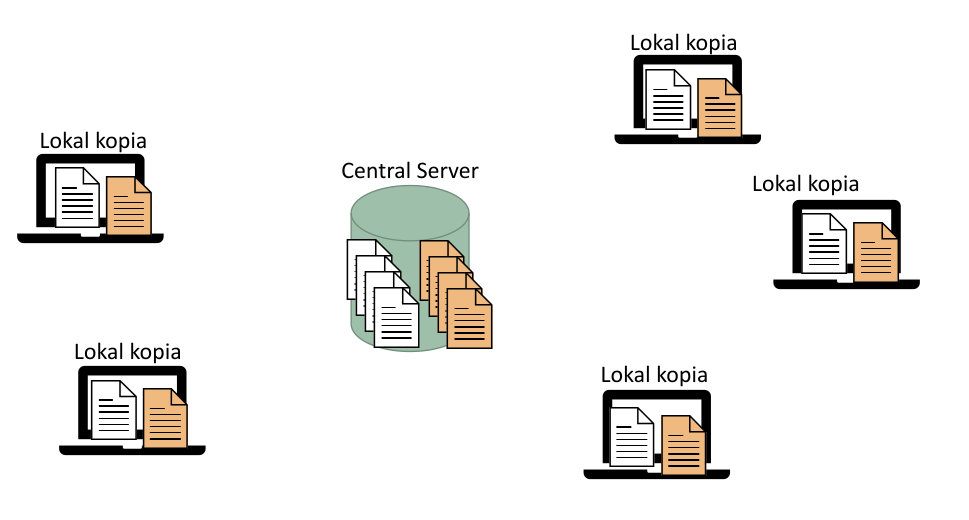
\includegraphics[width=0.80\textwidth]{figs/fig1_central_model.png}
    \end{center}
\end{frame}

\begin{frame}
    \frametitle{Typer av versionshanteringssystem (2/2)}

    \begin{block}{Distribuerade system}
        \begin{itemize}
            \ii{Ingen central server -- varje användare är en \enquote{nod} i systemet.}
            \ii{Varje användare har en lokal kopia av hela projektets historik.}
            \ii{Kommandon: \emph{clone} (kopiera hela repository), \emph{checkout} och \emph{commit} (men annorlunda), och \emph{push/pull} (synkronisera ändringar).}
            \ii{Exempel: Git, Mercurial}
        \end{itemize}
    \end{block}

\end{frame}

\begin{frame}
    \frametitle{Distrubuerad versionshantering}

    \begin{center}
        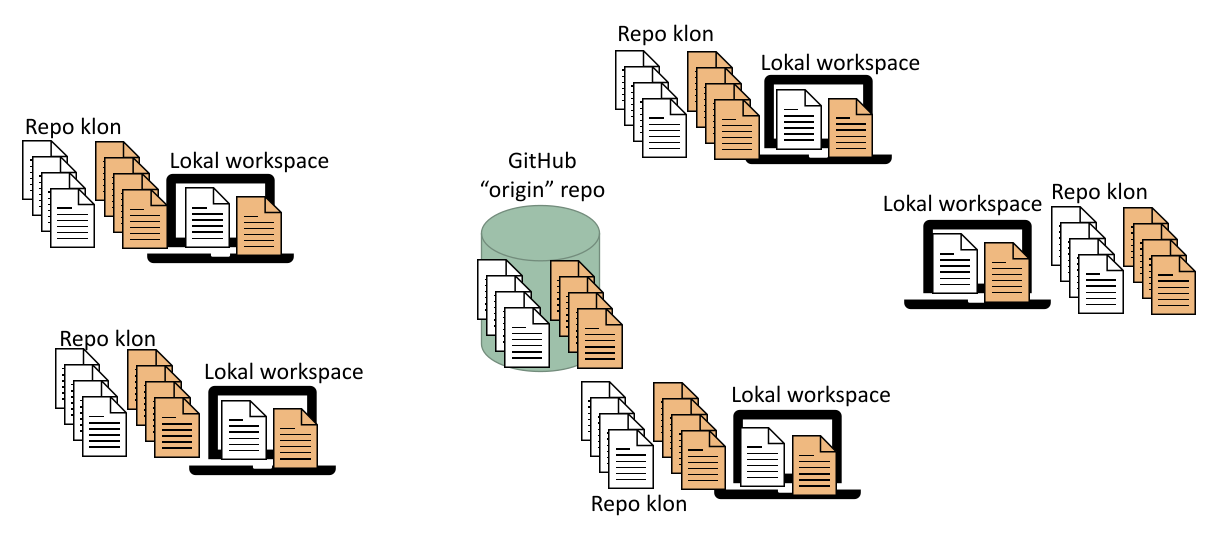
\includegraphics[width=\textwidth]{figs/fig2_git_model.png}
    \end{center}
\end{frame}

\begin{frame}
    \frametitle{Introduktion till Git}

    \begin{itemize}
        \ii{\emph{Git} är ett distribuerat versionshanteringssystem.}
        \ii{Utvecklat av Linus Torvalds 2005. \url{https://github.com/git/git}}
        \ii{Designat för snabb hantering av projekt med många bidragsgivare.}
        \ii{Används av de flesta moderna mjukvaruprojekt och open source-projekt.}
        \ii{Ger full kontroll över historik, branchning, och sammanslagning av ändringar (\emph{merging}).}
    \end{itemize}

    \blankline
    \ti{Testa: \code{git rev-list --max-parents=0 HEAD}}

\end{frame}

\begin{frame}
    \frametitle{Git vs. GitHub: Vad är skillnaden?}

    \begin{block}{Git}
        \begin{itemize}
            \ii{Ett \emph{verktyg} för versionshantering som körs lokalt på din dator.}
        \end{itemize}
    \end{block}

    \begin{block}{GitHub}
        \begin{itemize}
            \ii{En \emph{tjänst} för att hosta Git-repositories online.}
            \ii{Underlättar samarbete med andra utvecklare genom att erbjuda funktioner som pull requests, issues och projektöversikt.}
            \ii{Använder Git internt för att hantera repositories, precis som lokala installationer av Git.}
        \end{itemize}
    \end{block}

\end{frame}

\begin{frame}
    \frametitle{Grundläggande Git-kommandon}

    \begin{description}
        \di{git init}{Initierar ett nytt Git-repository lokalt.}
        \di{git clone}{Kopierar ett existerande repository (t.ex. från GitHub) till din dator.}
        \di{git add}{Lägger till ändringar i staging-området inför nästa commit.}
        \di{git commit}{Sparar ändringar lokalt med en beskrivande kommentar.}
        \di{git push}{Laddar upp dina lokala ändringar till ett fjärrrepository (t.ex. GitHub).}
        \di{git pull}{Hämtar och integrerar ändringar från ett fjärrrepository.}
    \end{description}

\end{frame}


\begin{frame}
    \frametitle{Git-modellen}

    \begin{itemize}
        \ii{\emph{Workspace}: En vanlig mapp på datorn där du jobbar med filer.}
        \ii{\emph{Staging Area}: En "kopia" av workspace där du förbereder ändringar inför nästa sparning.}
        \ii{\emph{Repository}: Ett arkiv som lagrar alla tidigare versioner av projektet.}
    \end{itemize}

    \begin{center}
        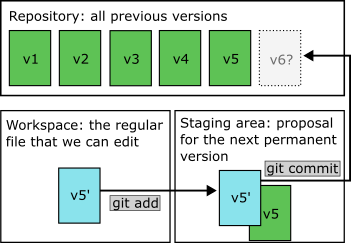
\includegraphics[height=.5\textheight]{figs/model-add-commit.png}
    \end{center}

\end{frame}

\begin{frame}
    \frametitle{Vad är en Commit?}

    \begin{minipage}{0.7\textwidth}
        \begin{itemize}
            \ii{En \emph{commit} är en "ögonblicksbild" (\emph{snapshot}) av projektet vid ett specifikt tillfälle.}
            \ii{Innehåller alla ändringar som gjorts sedan den senaste commiten.}
            \ii{Varje commit refererar till sin(a) föregångare och skapar en historik.}
            \ii{Bildar en graf av versioner som visar projektets utveckling över tid.}
        \end{itemize}
    \end{minipage}
    \hspace{.05\textwidth}
    \begin{minipage}{0.20\textwidth}
        \begin{center}
            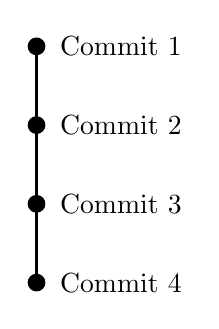
\begin{tikzpicture}
                % Draw the vertical line
                \draw[thick] (0, 0) -- (0, 3);

                % Draw the commit nodes
                \foreach \y in {0, 1, 2, 3} {
                        \filldraw (0, \y) circle (3pt);
                    }

                % Label the commits
                \node[right, xshift=5pt] at (0, 3) {Commit 1};
                \node[right, xshift=5pt] at (0, 2) {Commit 2};
                \node[right, xshift=5pt] at (0, 1) {Commit 3};
                \node[right, xshift=5pt] at (0, 0) {Commit 4};
            \end{tikzpicture}

        \end{center}
    \end{minipage}

\end{frame}

\begin{frame}
    \frametitle{Grenar (\emph{Branches})}

    \begin{minipage}{0.7\textwidth}

        \ti{Man kan skapa parallella utvecklingsgrenar, som sedan kan slås samman (\emph{merge}) med huvudgrenen igen.}

        \begin{itemize}
            \ii{Varför vill man göra det?}
            \ii{Vilka problem kan uppstå?}
        \end{itemize}
    \end{minipage}
    \hspace{.05\textwidth}
    \begin{minipage}{0.20\textwidth}
        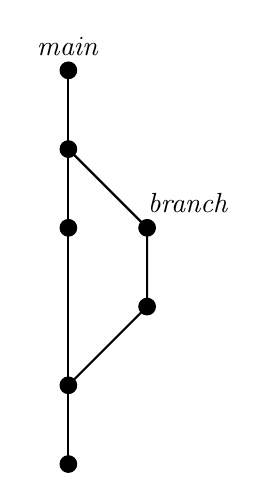
\begin{tikzpicture}
            % Rita huvudgrenen (main)
            \draw[thick] (0, 0) -- (0, 5);
            \foreach \y in {0, 1, 3, 4, 5} {
                    \filldraw (0, \y) circle (3pt);
                }
            \node[above, yshift=2pt] at (0, 5) {\emph{main}};

            % Rita parallellgrenen (branch)
            \draw[thick] (0, 4) -- (1, 3) -- (1, 2) -- (0, 1);
            \foreach \y in {2, 3} {
                    \filldraw (1, \y) circle (3pt);
                }
            \node[above, yshift=2pt, xshift=15pt] at (1, 3) {\emph{branch}};
        \end{tikzpicture}
    \end{minipage}

\end{frame}

\begin{frame}
    \frametitle{Varför grenar (\emph{branches})?}

    \begin{itemize}
        \ii{Grenar = parallella vägar; sidospår utan att störa huvudvägen.}
        \ii{Arbeta på olika delar av projektet samtidigt, utan att störa varandra.}
        \ii{Testa nya funktioner, experimentera säkert.}
        \ii{Skapa snabb fix för fel utan att stoppa ny utveckling.}
        \ii{Branches i Git är lätta att skapa och använda!}
    \end{itemize}

\end{frame}

\begin{frame}
    \frametitle{Vilka problem kan uppstå?}

    \begin{itemize}
        \ii{\emph{Merge}: Git kombinerar ändringar från olika grenar automatiskt.}
        \ii{\emph{Merge-konflikt}: Uppstår när Git inte kan avgöra hur vissa ändringar ska kombineras.}
        \ii{Konflikter sker ofta när samma del av en fil ändrats på flera grenar.}
        \ii{Exempel: Flera redigerar samma rad, eller ändrar/byter namn på samma filer.}
        \ii{Konflikter måste lösas manuellt för att slutföra en \emph{merge}.}
    \end{itemize}

\end{frame}

\begin{frame}[fragile]
    \frametitle{Exempel: Merge-konflikt i källkoden}

    \begin{block}{\small Kod före merge}
        \begin{GobbleCode}[0pt]{10}
            def greet(): String = {
                "Hello, world!"
            }
        \end{GobbleCode}
    \end{block}

    \begin{block}{\small Kod efter merge (med konflikt)}
        \begin{GobbleCode}[0pt]{10}
            def greet(): String = {
            <<<<<<< HEAD
                "Hello, world!"
            =======
                "Hi, everyone!"
            >>>>>>> branch
            }
        \end{GobbleCode}
    \end{block}

    \begin{itemize}
        \ii{Konflikten visas med \texttt{<<<<<<<}, \texttt{=======}, och \texttt{>>>>>>>}.}
        \ii{Utvecklaren måste välja vilken version som ska behållas eller kombinera dem manuellt.}
    \end{itemize}

\end{frame}


\begin{frame}[fragile]
    \frametitle{Ett större exempel}

    \begin{GobbleCode}[2pt]{6}
        object Main {
            def main(args: Array[String]): Unit = {
                println("Starting calculation...")
                println("Result: " + calculateSum(5, 10))
            }

            def calculateSum(a: Int, b: Int): Int = {
        <<<<<<< HEAD
                val sum = a + b
                println("Sum calculated: " + sum)
                sum
        =======
                val sum = a + b
                println("Calculating sum for: " + a + " and " + b)
                println("Sum is: " + sum)
                sum * 2 // Doubles the result
        >>>>>>> branch
            }
        }
    \end{GobbleCode}

\end{frame}

\begin{frame}
    \frametitle{Arbeta distribuerat med Git}

    \begin{itemize}
        \ii{\emph{Klona}: Kopiera ett repository från internet till din dator.}
        \ii{\emph{Pull}: Hämta ändringar från ett fjärrrepository.}
        \ii{\emph{Push}: Skicka dina ändringar till ett fjärrrepository.}
        \ii{\emph{Pull request}: Föreslå ändringar till ett repository.}
        \begin{itemize}
            \ii{Mycket vanligt i \emph{open source}-projekt.}
            \ii{Kallas ibland \emph{merge request}.}
        \end{itemize}
    \end{itemize}

\end{frame}

\begin{frame}
    \frametitle{Remote}

    \begin{itemize}
        \ii{Git använder termen \emph{remote}. Lokal \enquote{spegling} av fjärrrepository.}
        \ii{Standardnamn för remote är \texttt{origin}.}
        \ii{Möjligt att ha flera remotes för olika kopior av projektet.}
        \ii{Kolla med \texttt{git remote [-a, -v, -vv]}}
    \end{itemize}

\end{frame}

\begin{frame}
    \frametitle{Påminnelse - Context}

    \begin{center}
        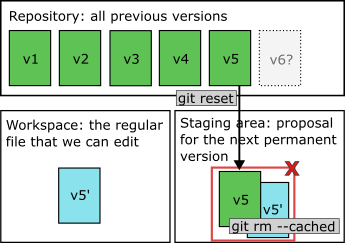
\includegraphics[height=.5\textheight]{figs/model-rm-reset.png}
    \end{center}

\end{frame}

\begin{frame}
    \frametitle{Local vs remote: commit och push}

    \begin{center}
        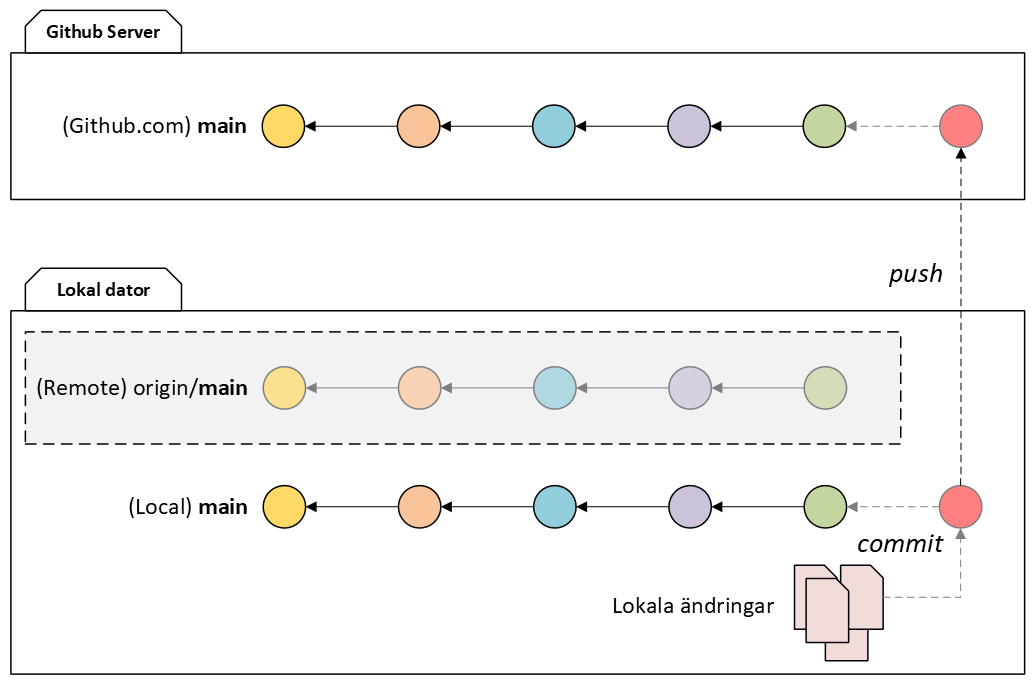
\includegraphics[width=.9\textwidth]{figs/local_remote_commit_push.png}
    \end{center}

\end{frame}

\begin{frame}
    \frametitle{Local vs remote: fetch och merge}

    \begin{center}
        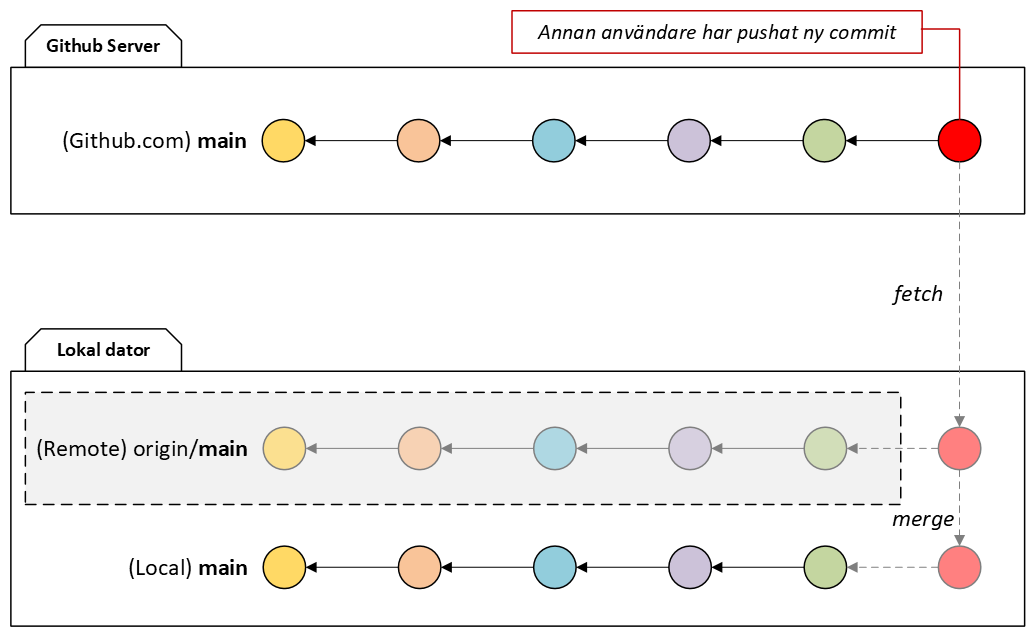
\includegraphics[width=.9\textwidth]{figs/local_remote_fetch_merge.png}
    \end{center}

\end{frame}

\begin{frame}
    \frametitle{Båda samtidigt!? -- push}

    \begin{center}
        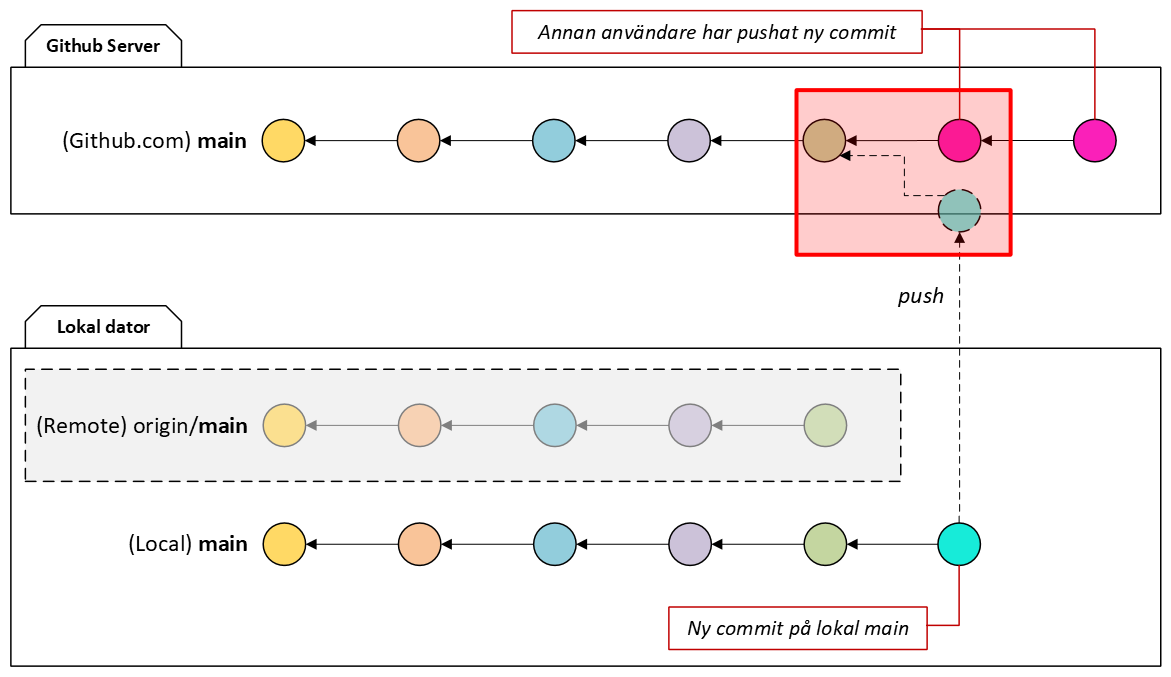
\includegraphics[width=\textwidth]{figs/local_remote_push_conflict.png}
    \end{center}

\end{frame}

\begin{frame}
    \frametitle{Båda samtidigt!? -- fetch}

    \begin{center}
        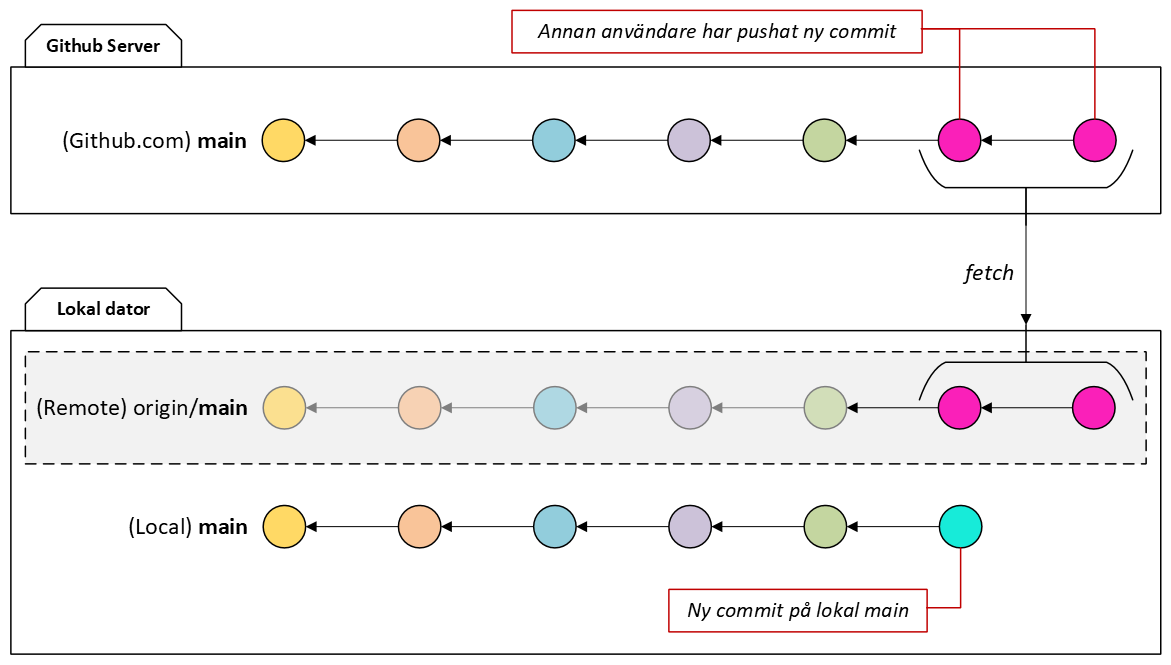
\includegraphics[width=\textwidth]{figs/local_remote_fetch_conflict.png}
    \end{center}

\end{frame}

\begin{frame}
    \frametitle{Båda samtidigt!? -- merge efter fetch}

    \begin{center}
        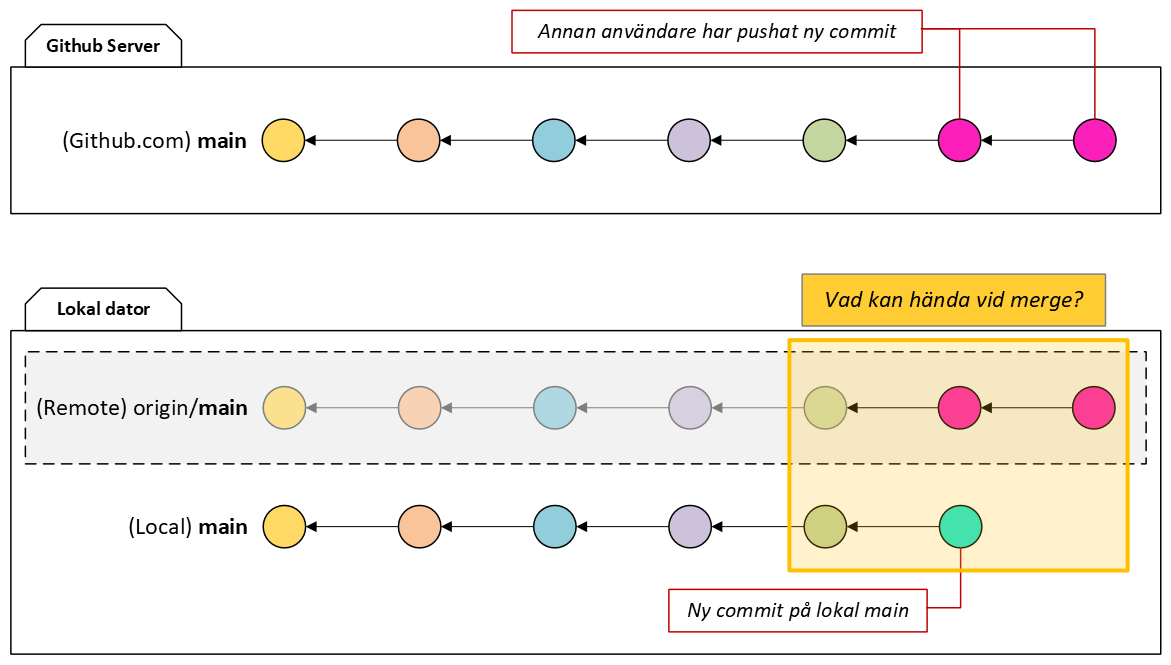
\includegraphics[width=\textwidth]{figs/local_remote_fetch_merge_conflict.png}
    \end{center}

\end{frame}


\begin{frame}
    \frametitle{Merge-situationer}

    \ti{Vad kan hända vid merge?}
    \begin{itemize}
        \ii{fast-forward merge}
        \ii{merge commit}
        \ii{konflikt}
        \ii{rebase}
    \end{itemize}

\end{frame}

\begin{frame}[t]
    \frametitle{Fast-forward merge}
    \vspace{-1.5em}
    \begin{center}
        \begin{tikzpicture}
            % Place the image at 50% scale
            \node (img) at (0, 0) {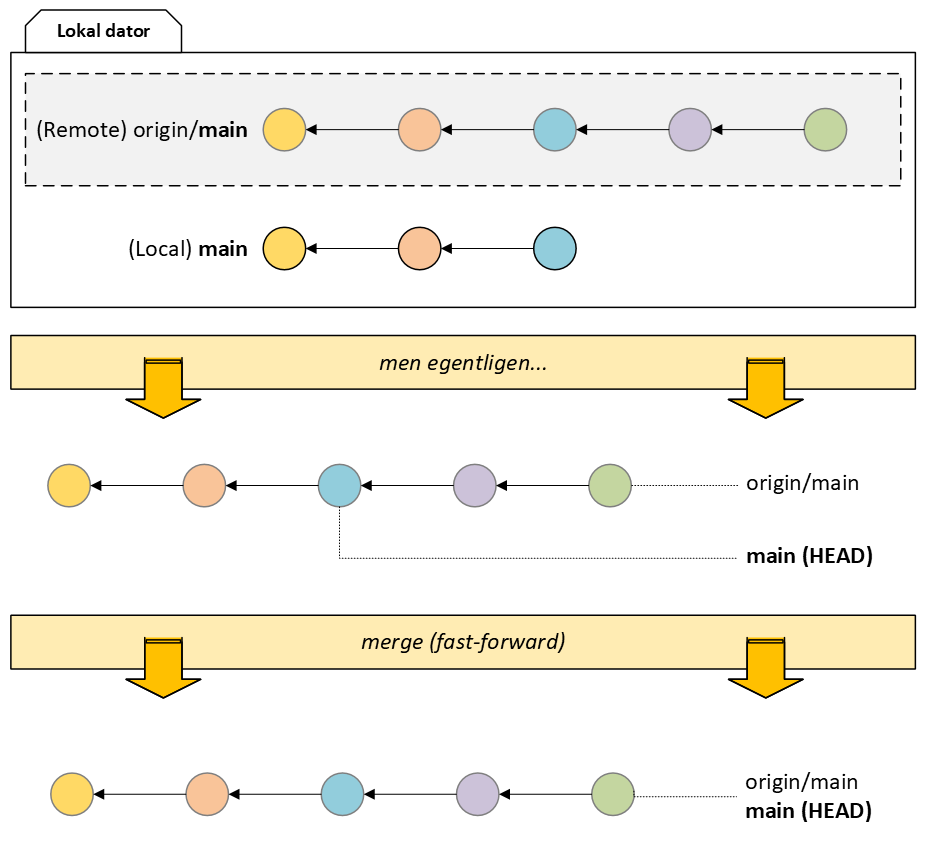
\includegraphics[scale=0.5]{figs/merge_case_ff.png}};

            % Only show partial overlays in the presentation mode
            \mode<beamer>{
                % Overlay 1: Cover the lower 2/3 of the image with a white box
                \only<1>{
                    \fill[white] ([yshift=-0.33\textheight]img.north west) rectangle (img.south east);
                }
                % % Overlay 2: Cover the lower 1/3 of the image with a white box
                \only<2>{
                    \fill[white] ([yshift=-0.6\textheight]img.north west) rectangle (img.south east);
                }
                % Overlay 3: Show the full image (no white box needed)
                \uncover<3>{
                    % No white box, full image visible
                }
            }
        \end{tikzpicture}
    \end{center}
\end{frame}

\begin{frame}[t]
    \frametitle{Vanlig merge -- skapar en \enquote{merge commit}}
    \begin{center}
        \begin{tikzpicture}
            % Place the image at 50% scale
            \node (img) at (0, 0) {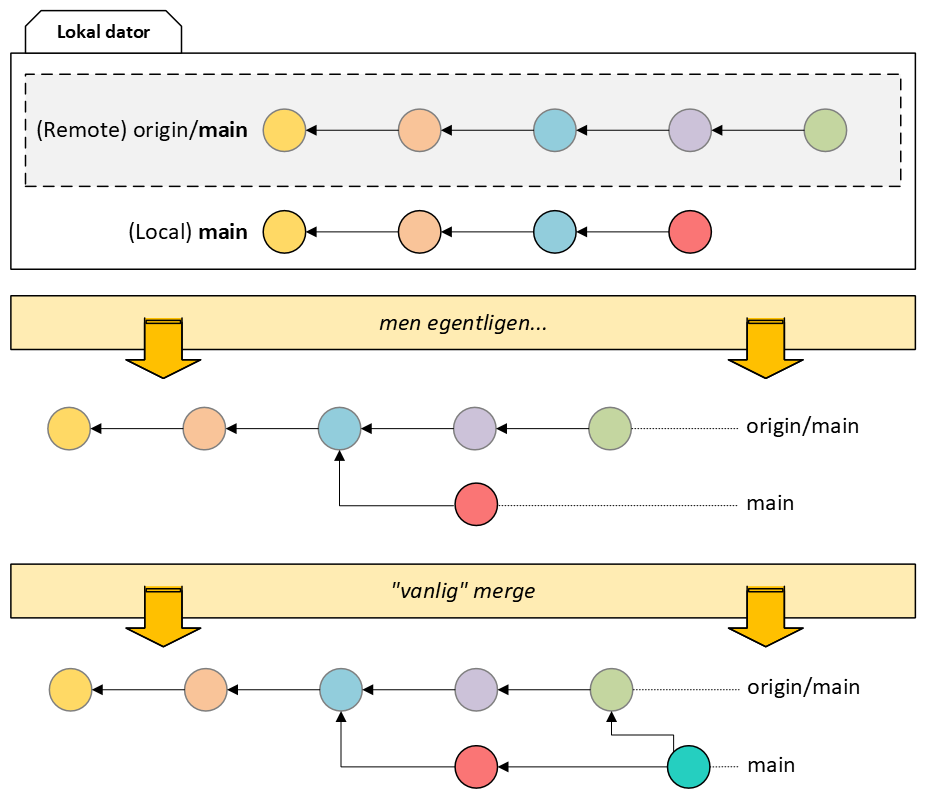
\includegraphics[scale=0.5]{figs/merge_case_commit.png}};

            % Only show partial overlays in the presentation mode
            \mode<beamer>{
                % Overlay 1: Cover the lower 2/3 of the image with a white box
                \only<1>{
                    \fill[white] ([yshift=-0.28\textheight]img.north west) rectangle (img.south east);
                }
                % % Overlay 2: Cover the lower 1/3 of the image with a white box
                \only<2>{
                    \fill[white] ([yshift=-0.55\textheight]img.north west) rectangle (img.south east);
                }
                % Overlay 3: Show the full image (no white box needed)
                \uncover<3>{
                    % No white box, full image visible
                }
            }
        \end{tikzpicture}
    \end{center}
\end{frame}

\begin{frame}
    \frametitle{Mergekonflikt}
    \ti{Vid konflikt, se föregående figur.}
    \begin{itemize}
        \ii{Om ändringarna i de två grenarna inte kan kombineras automatiskt, uppstår en konflikt.}
        \ii{Git markerar konflikter i filerna och pausar merge-processen.}
        \ii{Efter konflikten lösts, finns alltså ny ändringar i worspace\dots}
        \ii{...och du måste göra en ny commit för att slutföra merge.}
    \end{itemize}

\end{frame}

\begin{frame}[t]
    \frametitle{Rebase}
    \vspace{-.5em}
    \begin{center}
        \begin{tikzpicture}
            % Place the image at 50% scale
            \node (img) at (0, 0) {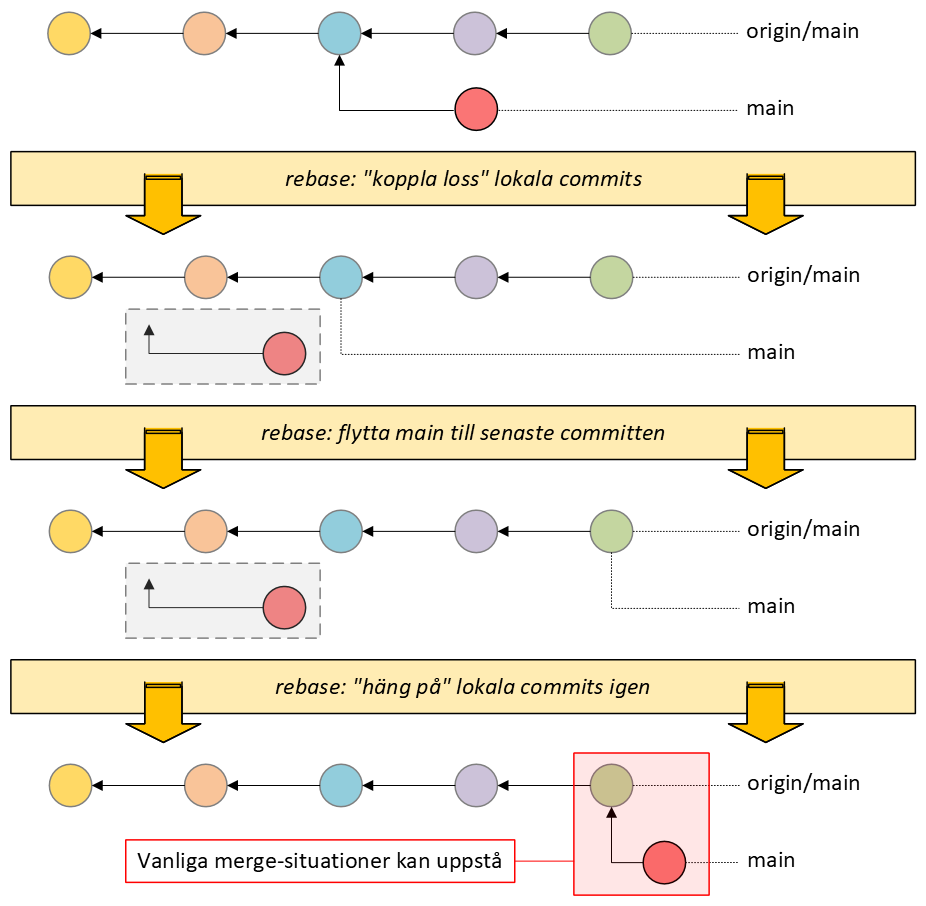
\includegraphics[scale=0.46]{figs/merge_case_rebase.png}};

            % Only show partial overlays in the presentation mode
            \mode<beamer>{
                % Overlay 1: Cover the lower 2/3 of the image with a white box
                \only<1>{
                    \fill[white] ([yshift=-0.14\textheight]img.north west) rectangle (img.south east);
                }
                % % Overlay 2: Cover the lower 1/3 of the image with a white box
                \only<2>{
                    \fill[white] ([yshift=-0.36\textheight]img.north west) rectangle (img.south east);
                }
                % % Overlay 3: Cover the lower 1/3 of the image with a white box
                \only<3>{
                    \fill[white] ([yshift=-0.59\textheight]img.north west) rectangle (img.south east);
                }
                % Overlay 4: Show the full image (no white box needed)
                \uncover<4>{
                    % No white box, full image visible
                }
            }
        \end{tikzpicture}
    \end{center}
\end{frame}



\begin{frame}
    \frametitle{Bra att veta}

    \begin{itemize}
        \ii{\code{HEAD} är en \emph{symbolisk referens} till den branch som är utcheckad i ditt workspace.}
        \ii{\enquote{Detatched HEAD} -- om du checkar ut en specifik commit, snarare än en branch.}
    \end{itemize}
\end{frame}

\begin{frame}
    \frametitle{Veckans laboration}

    \ti{På veckans laboration kommer ni:}
    \begin{itemize}
        \ii{Arbeta er igenom ett enkelt scenario som visar hur ni kan använda Git och Github för ett litet projekt.}
        \ii{Tänkt att kunna genomföras individuellt, men OK och uppmuntras till att samarbeta, speciellt i den sista delen av laborationen.}
    \end{itemize}

    \halfblankline
    \ti{Glöm inte att:}
    \begin{itemize}
        \ii{Installera Git på din egen dator.}
    \end{itemize}

\end{frame}

\begin{frame}
    \frametitle{Vad händer nu?}
    \begin{itemize}
        \ii{Läs avsnittet om Git i Scalakompendiet (Björn Regnell).}
        \ii{Se avsnitt 1.1, 1.2, 1.3, 1.6 samt 1.7 av youtube-serien \enquote{Git and GitHub for Poets}.}
        \ii{Läs kapitel 1, 2 och 3.1--3.2 i Pro Git-boken (Chacon \& Straub).}
        \ii{Länkar till materialet finns på kurshemsidan:

            \halfblankline
            \url{https://lunduniversity.github.io/pgk}}
    \end{itemize}

\end{frame}


\newpage

\title{\LaTeX}
\section{\LaTeX}

\begin{frame}[fragile=singleslide]
\label{latex}
\begin{block}{\centering\Large Föreläsning 2 --- \LaTeX}
Förberedelse inför laboration 2.

\begin{itemize}
\item Ordbehandling
\item \LaTeX
\item Mall för rapport
\item Dokumentstruktur: dokumentklasser, omgivningar, text, stycken, listor, tabeller, \ldots
\item Programlistor
\item Matematiska formler
\item Bilder
\end{itemize}
\end{block}
\end{frame} 

\begin{frame}[fragile=singleslide]
\frametitle{Ordbehandling}
De flesta moderna ordbehandlare, till exempel Microsoft Word,  fungerar 
enligt \textsc{WYSIWYG}-principen:

\blankline
\begin{center}
What You See Is What You Get
\end{center}

\blankline
Det innebär att det man ser på skärmen ser likadant ut som det som kommer
att skrivas på papperet: teckensnitt, storlekar, avstånd, \ldots

Det innebär också att det inte blir bättre än vad det ser ut
på skärmen (What You See Is \emph{All} You Get).
\end{frame} 

\begin{frame}[fragile=singleslide]
\frametitle{Layout av text}
I de flesta ordbehandlare finns det
formatmallar där man till exempel kan bestämma att alla rubriker på
en viss nivå ska ha ett visst utseende. Om man vill ändra
utseendet på alla rubriker så räcker det att ändra i mallen.

\blankline
Det brukar också finnas möjlighet till automatisk numrering av 
rubriker, automatisk generering av innehållsförteckning och 
sakregister och liknande. 

\blankline
När man skriver matematisk text använder man ofta en ekvationseditor
för att skriva de matematiska symbolerna. Ekvationseditorer är inte
enkla att använda, och slutresultatet brukar inte bli bra.
\end{frame} 

\begin{frame}[fragile=singleslide]
\frametitle{\LaTeX}
Med \LaTeX\ arbetar man på ett helt annat sätt: man skriver 
texten i en vanlig textfil och lägger
in \emph{kommandon} (''taggar'')  i texten som visar hur texten ska
formateras. Textfilen kan bli något svårläst, åtminstone innan man är van, men resultatet blir garanterat snyggt.

\blankline
Enkelt exempel:

\begin{exempel}
Pythagoras sats ser ut så
här: $a^2 + b^2 = c^2$.
\end{exempel} 

\code{\$}-tecknen anger att en matematisk formel börjar och slutar. 
\LaTeX\ vet då att variablerna a, b och c ska skrivas kursiva, hur stora
exponenterna ska vara och var de ska placeras, och hur
mycket mellanrum det ska vara mellan termerna.

\end{frame} 

\begin{frame}[fragile=singleslide]
\frametitle{Ett större exempel}
\begin{mexempel}
   If $f$ is continuous on the
   closed interval $a \leq x \leq b$
   and differentiable on the open
   interval $a < x < b$, then there
   exists a point
   $\xi$, $a < \xi < b$ such that
   \begin{displaymath}
      f(b) - f(a) = f'(\xi)(b -a).
   \end{displaymath}
\end{mexempel}

\end{frame} 

\begin{frame}[fragile=singleslide]
\frametitle{\LaTeX-historik}
Donald E. Knuth skrev 1977--1982 typsättningsprogrammet \TeX
\footnote{\TeX\ skrivs TeX i skrivmaskinsskrift och uttalas
''tech''.} 
eftersom han inte var nöjd med de möjligheter till typsättning
som fanns då.

\TeX\ är ett ''lågnivåspråk''. Leslie Lamport byggde på \TeX\ 
med ett makropaket som gör det möjligt för författaren av ett
dokument att koncentrera sig på den logiska strukturen hos
dokumentet och på själva texten i stället för på lågnivåtypsättningen. 
Resultatet
blev \LaTeX
\footnote{\LaTeX\ skrivs LaTeX i skrivmaskinsskrift och uttalas
''lah-tekh'' eller "lay-tekh".}.

En föregångare till \LaTeX, \emph{troff}, används fortfarande
ibland, till exempel till Unix man-sidor.
\end{frame} 

\begin{frame}[fragile=singleslide]
\frametitle{Arbeta med \LaTeX}
När man använder \LaTeX\ utgår man från en fil med text och kommandon. Filen ska ha tillägget \code{.tex}, till exempel \code{rapport.tex}. Sedan ''översätter'' man filen till \code{pdf}-format med programmet \code{pdflatex} och tittar på resultatet med en pdf-läsare, till exempel \code{evince}. Detta kan man naturligtvis göra genom att skriva kommandona för hand (\code{gedit rapport.tex}, \code{pdflatex rapport.tex}, \code{evince rapport.pdf}), men det är enklare att använda ett specialprogram. På studentdatorerna finns programmet \code{texmaker}. På Mac-datorer använder man t.ex. TeXShop eller TeXstudio som även finns för Windows.

\pindent I stället för att generera pdf-filer med \code{pdflatex} kan man generera dvi-filer (''device independent'') med programmet \code{latex} som man kan titta på med en ''dvi-läsare'' och sedan översätta till Postscript eller pdf. Numera använder de flesta \code{pdflatex}.
\end{frame} 

\begin{frame}[fragile=singleslide]
\frametitle{Mall för rapport}
\vspace{-2mm}
\bex 
\documentclass[a4paper]{article}
\usepackage[T1]{fontenc}
\usepackage[utf8]{inputenc}
\usepackage[swedish]{babel}
\usepackage{fancyvrb}
\fvset{tabsize=4}
\fvset{fontsize=\small}
\title{Programmeringsteknik\\
   Inlämningsuppgift 1}
\author{Xerxes Yngvesson\\
   dat14xyn@student.lu.se}
\date{2014--10--17}

\begin{document}
\maketitle

Här skriver man texten i
rapporten.
\end{document}
\end{verbatim}
\mex
\begin{center}
\LARGE Programmeringsteknik \\
\LARGE \ Inlämningsuppgift 1\\
\blankline
\large Xerxes Yngvesson \\
\large dat14xyn@student.lu.se\\
\large 2014--10--17
\end{center}
\vspace{1cm}
Här skriver man texten i
rapporten.
\eex
\end{frame} 

\begin{frame}[fragile=singleslide]
\frametitle{Dokumentklasser och omgivningar}
\verb+{article}+ är en \emph{dokumentklass} (den man oftast använder). 
Andra dokumentklasser är \verb+{report}+,
\verb+{book}+, \verb+{letter}+ och \verb+{beamer}+ (beamer används för overheadbilder). En dokumentklass
påverkar utseendet på hela dokumentet.

\blankline
\verb+\begin{document}+ definierar starten på en \emph{omgivning},
\verb+\end{document}+ slutet på omgivningen. En omgivning påverkar
utseendet på den del av dokumentet som ingår i omgivningen.
Vi kommer att se exempel på andra omgivningar senare. 
\end{frame} 

\begin{frame}[fragile=singleslide]
\frametitle{Löpande text}
Radslut och antal mellanslag mellan ord har ingen betydelse,
\LaTeX\ formaterar så att det blir snyggt. En
eller flera blanka rader ger ett nytt stycke. Exempel:

\bex
Det här
är en text som jag
har    skrivit. Det är
en lång text med flera
rader.

Här börjar det ett
nytt stycke i texten.
\end{verbatim}
\mex
Det här
är en text som jag
har    skrivit. Det är
en lång text med flera
rader.

\hspace{1em}Här börjar det ett
nytt stycke i texten.
\eex
\end{frame} 

\begin{frame}[fragile=singleslide]
\frametitle{Rubriker}
\LaTeX\ numrerar rubriker automatiskt. Man anger en rubrik med
\verb+\section+ eller \verb+\subsection+.

\bex 
\section{Inledning}
\section{Utförande}
\subsection{Del 1}
\subsection{Del 2}
\section{Slutsatser}
\end{verbatim}
\mex
{\Large\bfseries 1 Inledning} \\[1ex]
{\Large\bfseries 2 Utförande} \\[1ex]
{\large\bfseries 2.1 Del 1} \\[1ex]
{\large\bfseries 2.2 Del 2} \\[1ex]
{\Large\bfseries 3 Slutsatser}
\eex

\end{frame} 

\begin{frame}[fragile=singleslide]
\frametitle{Ändra textens utseende}
Det finns många kommandon för att ändra utseende på texten. Två 
sådana kommandon  är \verb+\emph+ för att betona text och \verb+\texttt+
för att skriva med skrivmaskinstypsnitt. Exempel:

\begin{exempel}
Här skriver jag något
\emph{viktigt}. Och 
i Java har vi använt
klassen \texttt{Square}.
\end{exempel}

Det finns också kommandon för fetstil, lutande text, osv, och för att
ändra storlek på texten. Använd sparsamt!
\end{frame} 

\begin{frame}[fragile=singleslide]
\frametitle{Specialtecken}
Med tecknet \code{\%} inleder man en kommentar som sträcker sig till slutet av raden.

\blankline
En del tecken används för kommandon och måste skrivas på speciellt sätt:

\begin{Code}
\$ \% \_ \# \& \{ \} \textbackslash
\end{Code}

Det finns streck, mellanrum och punkter av olika slag:

\begin{exempel}
DoD-kursen pågår under vecka
1--3 av läsperiod ht1. Tyvärr 
är den inte längre \ldots

\quad Telefon: 046--222~80~38.
Dagens datum: \today.
\end{exempel}
\end{frame} 

\begin{frame}[fragile=singleslide]
\frametitle{Fotnoter}
Fotnoter är lätta att skriva:

\bex 
Om man använder \LaTeX
\footnote{uttalas 
''lah-tekh''} så
blir det bra. Alla rapporter
blir automatiskt snyggt
utformade.
\end{verbatim}
\mex
Om man använder \LaTeX
\footnote{uttalas 
''lah-tekh''} så
blir det bra. Alla rapporter
blir automatiskt snyggt
utformade.
\eex

Fotnoter numreras automatiskt 1,2,\ldots 
Fast här blev ''numret'' på fotnoten ''a'' av olika anledningar.
Observera att man skriver två apostrofer (\verb+''+) i stället
för citationstecken (\code{"}).
\end{frame} 

\begin{frame}[fragile=singleslide]
\frametitle{Listor}
Punktlistor är enkla:

\begin{exempel}
\begin{itemize}
  \item första punkten
  \item här kommer den andra 
  punkten i listan
\end{itemize}
\end{exempel}

Numrerade listor är lika enkla:

\begin{exempel}
\begin{enumerate}
  \item första punkten
  \item här kommer den andra
  punkten i listan
\end{enumerate}
\end{exempel}

OBS! Pga hur detta dokument är formaterat så får listelementen inga punkter eller siffror, men i den vanliga dokumentklassen \code{\{article\}} blir det som förväntat.
% I detta dokument används dokumentklassen \code{beamer}, och där blir numren siffror i cirklar. I den vanliga dokumentklassen \code{\{article\}} blir numren 1., 2., \ldots
\end{frame} 

\begin{frame}[fragile=singleslide]
\frametitle{Definitioner}
\begin{exempel}
Några klasser som vi använder:

\begin{description}
\item[SimpleWindow] Beskriver ett
enkelt ritfönster
\item[Scanner] Inläsning från 
tangentbordet
\item[Random] Slumptal
\end{description}
\end{exempel}

I dokumentklassen \code{article} blir det något annorlunda layout på definitioner. Använd en \code{tabular}-omgivning med kolumnspecifikationen \code{p\{bredd\}} för att få layout som liknar den ovan.
\end{frame} 

\begin{frame}[fragile=singleslide]
\frametitle{Tabeller}
En tabell där den första kolumnen är vänsterinpassad (\code{l}), den 
andra centrerad (\code{c}) och den tredje högerinpassad (\code{r}). \code{\&} avgränsar kolumnerna, 
\verb+\\+ betyder ny rad, \verb+~+ är ett ''hårt'' blanktecken. \verb+\hline+ är ett streck.

\bex
\begin{tabular}{lcr}
  Produkt  & Typ    & Pris    \\
  \hline
  Skruvar  & stora  & 0.18~kr \\
  Muttrar  & M16    & 0.38~kr \\
  Spikar   & 12~tum & 0.12~kr
\end{tabular}
\end{verbatim}
\mex
\begin{tabular}[t]{lcr}
  Produkt  & Typ    & Pris    \\
  \hline
  Skruvar  & stora  & 0.18~kr \\
  Muttrar  & M16    & 0.38~kr \\
  Spikar   & 12~tum & 0.12~kr
\end{tabular}
\eex
\end{frame} 

\begin{frame}[fragile=singleslide]
\frametitle{Flytande tabeller}
Med en \verb+\table+-omgivning skapar man en tabell med en förklarande
text och ett nummer. \LaTeX\ placerar tabellen där det är 
lämpligt.

\bex
\begin{table}
\begin{tabular}{lcr}
  Produkt  & Typ    & Pris    \\
  \hline
  Skruvar  & stora  & 0.18~kr \\
  Muttrar  & M16    & 0.38~kr \\
  Spikar   & 12~tum & 0.12~kr
\end{tabular}
\caption{Våra produkter}
\end{table}
\end{verbatim}
\mex
\begin{tabular}[t]{lcr}
  Produkt  & Typ    & Pris    \\
  \hline
  Skruvar  & stora  & 0.18~kr \\
  Muttrar  & M16    & 0.38~kr \\
  Spikar   & 12~tum & 0.12~kr
\end{tabular}
\begin{center}
{Tabell 7. Våra produkter}
\end{center}
\eex
\end{frame} 

\begin{frame}[fragile=singleslide]
\frametitle{Att referera till etiketter}
Om man sätter en etikett på en tabell kan man referera till den
från texten. Exempel: 

\bex
\begin{table}
\begin{tabular}{lcr}
  Produkt  & Typ    & Pris    \\
  \hline
  Skruvar  & stora  & 0.18~kr \\
\end{tabular}
\caption{Våra produkter}
\label{produkter}
\end{table}
Senare i texten: våra produkter
finns i tabell~\ref{produkter}.
\end{verbatim}
\mex
\begin{tabular}[t]{lcr}
  Produkt  & Typ    & Pris    \\
  \hline
  Skruvar  & stora  & 0.18 kr \\
\end{tabular}
\begin{center}
{Tabell 7. Våra produkter}
\end{center}
Senare i texten: våra produkter
finns i tabell~7.
\eex
Figurer hanteras likadant som tabeller, i en 
\verb+\figure+-omgivning.
\end{frame} 

\begin{frame}[fragile=singleslide]
\frametitle{Programlistor}
För att infoga en programlista i en rapport använder man
kommandot \verb+\VerbatimInput{filnamn}+ från paketet
\texttt{fancyvrb}. Man bör \emph{inte} använda ''standard''-
kommandot \verb+\verbatiminput+ eftersom det kommandot
ignorerar alla tabulatortecken i programmet, och det medför att
indragningarna försvinner.

\bex
\usepackage{fancyvrb}
\fvset{tabsize=4}
\fvset{fontsize=\small}

\VerbatimInput{Point.java}
\end{verbatim}
\mex
%\vspace{-30pt}
\begin{verbatim}
class Point {
    private int x;
    private int y;

    public Point(int x, int y) {
        this.x = x;
        this.y = y;
    }
}
\end{verbatim}
\eex
\end{frame} 

\begin{frame}[fragile=singleslide]
\frametitle{Öka eller minska avstånd}
Ibland behöver man öka avståndet i vertikalled mellan två avsnitt i texten, till exempel före eller efter en tabell. Det kan man göra med kommandot \verb/\vspace{längd}/, där längden kan anges i millimeter eller punkter eller något annat som \LaTeX\ känner igen. Längden kan vara negativ om man vill minska avståndet. Det finns också specialkommandon för att lägga in ett litet, mellanstort och stort avstånd:

\begin{Code}
\smallskip  \medskip  \bigskip
\end{Code}

Man kan öka eller minska horisontellt avstånd med \verb/\hspace{längd}/.
\end{frame} 

\begin{frame}[fragile=singleslide]
\frametitle{Matematiska formler}
\LaTeX\ är \emph{mycket} bra på att formatera matematisk text. 
Alla (tror jag) artiklar och böcker som innehåller matematiska formler 
är skrivna med \LaTeX. Man kan skriva
formler antingen inuti löpande text eller på en egen rad:
\begin{itemize}
\item I texten: formeln inleds med \code{\$} och avslutas med \code{\$}.
\item På egen rad: formeln inleds med \verb+\begin{displaymath}+
och avslutas med \verb+\end{displaymath}+.
\verb+\begin{equation}+ och \verb+\end{equation}+ ger samma
resultat men formeln numreras. Med \verb+\label+ och \verb+\ref+
kan man etikettera och referera till ekvationer.
\end{itemize}
\end{frame} 

\begin{frame}[fragile=singleslide]
\frametitle{Enkla formler}
\begin{mexempel}
Formeln $x=3y-2$ står 
inne i texten. Däremot
står
\begin{displaymath}
  x=3y-2
\end{displaymath}
för sig själv precis som
\begin{equation}
  x=3y-2
  \label{xochy}
\end{equation}
I ekvation~\ref{xochy} fann
vi att \ldots
\end{mexempel}
\end{frame} 

\begin{frame}[fragile=singleslide]
\frametitle{Symboler, index}
\begin{mexempel}
\begin{displaymath}
\alpha \leq \pi \approx 3.141592654
\end{displaymath}
\end{mexempel}

\vspace{1cm}

\begin{mexempel}
\begin{displaymath}
x_{k+1}=x_{k}-f(x_{k})/f'(x_{k})
\end{displaymath}
\end{mexempel}
\end{frame} 

\begin{frame}[fragile=singleslide]
\frametitle{Exponenter, rötter}
\begin{mexempel}
\begin{displaymath}
e^x = 1+x+x^2/2!+x^3/3!+\cdots
\end{displaymath}
\end{mexempel}

\vspace{1cm}

\begin{mexempel}
\begin{displaymath}
x_{1,2}=\frac{p}{2}\pm
\sqrt{\frac{p^2}{4}-q}
\end{displaymath}
\end{mexempel}

\end{frame} 



\begin{frame}[fragile=singleslide]
\frametitle{Integraler, summor}
\begin{mexempel}
\begin{displaymath}
\int_{-\infty}^{\infty}
e^{-x^2} dx
\end{displaymath}
\end{mexempel}

\vspace{1cm}

\begin{mexempel}
\begin{displaymath}
\sum_{k=1}^n\frac{1}{a_k}
\end{displaymath}
\end{mexempel}

\end{frame} 

\begin{frame}[fragile=singleslide]
\frametitle{Funktioner}
\begin{mexempel}
\begin{displaymath}
  \sin^2 x + \cos^2 x = 1
\end{displaymath}
\end{mexempel}
\end{frame} 

\begin{frame}[fragile=singleslide]
\frametitle{Matriser, parenteser}
\begin{mexempel}
\begin{displaymath}
A=\left(
\begin{array}{cccc}
a_{11} & a_{12} & \cdots & a_{1n}\\
a_{21} & a_{22} & \cdots & a_{2n}\\
\vdots & \vdots & \ddots & \vdots\\
a_{n1} & a_{n2} & \cdots & a_{nn}\\
\end{array}
\right)
\end{displaymath}
\end{mexempel}
\end{frame} 

\begin{frame}[fragile=singleslide]
\frametitle{Bilder}
Bilder kan inkluderas i \LaTeX-dokument om de är i formatet
\code{pdf}, \code{jpeg} eller \code{png} (\texttt{eps} om man använder \code{latex}). Man måste använda paketet \texttt{graphicx} (eller \code{graphics}).
\vspace{20mm}
\bex
\usepackage{graphicx}


\includegraphics[height=40mm]{images/bild.pdf}
\end{verbatim}
\mex
  \vspace{-25mm}\hspace{15mm}
  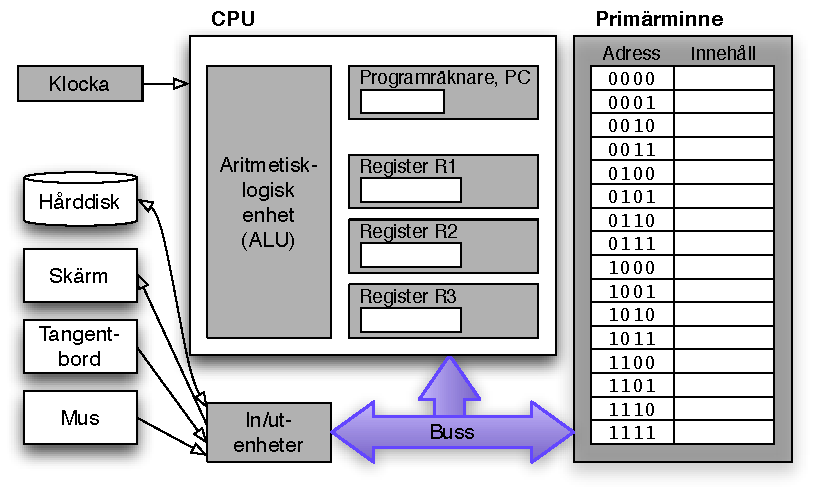
\includegraphics[height=30mm]{images/enkelmodell.pdf}
\eex

ImageMagick-programmet \texttt{convert} kan konvertera
från och till de flesta bildformat:
\begin{verbatim}
   convert bild.fig bild.pdf
\end{verbatim}
\end{frame} 

\begin{frame}[fragile=singleslide]
\frametitle{Egna kommandon}
Man kan lätt definiera egna kommandon, till exempel ett kortare namn
för en text som man använder ofta. Kommandon kan ha parametrar.

\vspace{10mm}

\begin{mexempel}
\newcommand{\java}[1]
{\texttt{#1}}

Klasser: \java{Random}, 
\java{Scanner} och 
\java{PrintStream}.
\end{mexempel}

\vspace{10mm}

Man kan definiera om existerande kommandon med
\verb+\renewcommand+. Det kan ställa till förvirring, så
gör inte det.
\end{frame} 

%\begin{frame}[fragile=singleslide]
%\frametitle{\LaTeX\ på egen dator}
%
%En sammanfattning av LaTeX-installationer finns på \url{www.latex-project.org}, sidan Getting LaTeX.
%
%\begin{description}
%\item[Linux] LaTeX kanske redan finns på datorn; hämtas annars med den vanliga pakethanteraren.
%\item[Mac] Använd MacTeX (bygger på TeXLive, som uppdateras varje år).
%\item[Windows] proTeXt verkar vara enklast.
%\end{description}
%
%Som IDE rekommenderas Texmaker (\url{www.xm1math.net/texmaker}) eller TeXShop (bara för Mac, \url{www.texshop.org}).
%\end{frame} 



\newpage

\title{Maskinkod}
\section{Maskinkod}


\begin{frame}
    \begin{block}{\centering\Large Föreläsning \arabic{section} --- Maskinkod}
        Förberedelse inför laboration 4.

        \begin{itemize}
            \item Vad är en dator?
            \item Binära tal.
            \item CPU och Minne.
            \item Maskinkod och instruktioner.
            \item Assembly-språk.
            \item Kompilerare och tolkar.
            \item c3pu (labförberedelse).
        \end{itemize}
    \end{block}
\end{frame}

\begin{frame}[fragile=singleslide]
    \frametitle{Bakgrund}
    \begin{columns}
        \begin{column}{0.75\textwidth}
            \begin{block}{Varför lära sig Maskinkod?}
                \begin{itemize}
                    \item \textbf{Effektiv Problemlösning:} Förstå hur datorer utför uppgifter kan leda till snabbare och mer effektiva lösningar när du programmerar.
                    \pause
                    \item \textbf{Förbättrade felsökningsfärdigheter:} Kunskap om maskinkod kan avslöja djupliggande orsaker till buggar, vilket gör det enklare att fixa komplexa problem.
                    \pause
                    \item \textbf{Bättre teknikval:} Grundläggande förståelse för maskinkod kan vägleda dig i val av hårdvara och optimeringar, likt valet av motor för en bil baserat på användningsområde.
                    \pause
                    \item \textbf{Innovativt tänkande:} Förståelsen för datorns fundamentala operationer möjliggör kreativa och nyskapande tekniklösningar.
                \end{itemize}
            \end{block}
        \end{column}
        \begin{column}{0.25\textwidth}
            \begin{center}
                \begin{tikzpicture}
                    \node (hl) [rectangle, draw, fill=blue!20, text width=6em, text centered, minimum height=2em] {Högnivåspråk};
                    \node (al) [rectangle, draw, fill=green!20, below=of hl, text width=6em, text centered, minimum height=2em] {Assembly};
                    \node (mc) [rectangle, draw, fill=red!20, below=of al, text width=6em, text centered, minimum height=2em] {Maskinkod};
                    \node (hw) [rectangle, draw, fill=orange!20, below=of mc, text width=6em, text centered, minimum height=2em] {Hårdvara};

                    \draw[->] (hl) -- (al);
                    \draw[->] (al) -- (mc);
                    \draw[->] (mc) -- (hw);
                \end{tikzpicture}
            \end{center}
        \end{column}
    \end{columns}
\end{frame}


\begin{frame}[fragile=singleslide]
    \frametitle{Vad är en dator?}
    \begin{columns}[T] % The [T] option is used to align the columns content at the top
        \begin{column}{0.6\textwidth}
            \begin{block}{Komponenter}
                \begin{itemize}
                    \item \textbf{CPU:} Datorns hjärna, innehåller ALU, kontrollenhet, och internminne (cache).
                    \pause
                    \item \textbf{Minne:} Lagring av data och instruktioner. RAM och permanent lagring (t.ex., hårddisk).
                    \pause
                    \item \textbf{I/O-enheter:} För inmatning och utmatning, t.ex., mus, tangentbord, skärm.
                \end{itemize}
            \end{block}
            \begin{block}{Programvara vs. Hårdvara}
                \begin{itemize}
                    \item \textbf{Hårdvara:} Fysiska delarna av datorn.
                    \item \textbf{Programvara:} Instruktioner för att utföra uppgifter.
                \end{itemize}
            \end{block}
        \end{column}
        \begin{column}{0.4\textwidth}
            \begin{center}
                \begin{tikzpicture}[scale=0.8, every node/.style={scale=0.8}]
                    % Define CPU and its internal components
                    \node (cpu) [rectangle, draw, fill=blue!20, minimum height=9.2em, minimum width=9.5em, rounded corners, align=center, label=above:CPU] {};
                    \node (cu) [rectangle, draw, fill=green!30, below=.5em of cpu.north, minimum height=1.5em, minimum width=9em, align=center] {Control Unit};
                    \node (alu) [rectangle, draw, fill=red!30, below=.5em of cu, minimum height=1.5em, minimum width=9em, align=center] {ALU};
                    \node (pm) [rectangle, draw, fill=orange!40, below=.5em of alu, minimum height=1.5em, minimum width=9em, align=center] {Primary Cache};
                    \node (sm) [rectangle, draw, fill=yellow!40, below=.2em of pm, minimum height=1.5em, minimum width=9em, align=center] {Secondary Cache};
                    
                    % Define I/O Devices
                    \node (io) [rectangle, draw, fill=gray!30, below=of cpu, minimum height=3em, minimum width=9.5em, rounded corners, align=center, label=above:I/O Devices] {Mouse, Keyboard,\\Screen, etc.};

                    % Define RAM
                    \node (ram) [rectangle, draw, fill=purple!40, left=of cpu, yshift=-3.1em, xshift=3em, minimum height=15.5em, minimum width=3em, rounded corners, align=center, label=above:RAM] {};

                \end{tikzpicture}
            \end{center}
        \end{column}
    \end{columns}
    
\end{frame}

\begin{frame}[fragile=singleslide]
    \frametitle{Binära tal - Introduktion}
    \begin{block}{Olika talsystem}
        \begin{itemize}
            \item Talsystem används för att representera tal med symboler.
            \item Decimal (bas 10) - vanligaste, använder siffror 0-9.
        \end{itemize}
    \end{block}
    \begin{block}{Binärt talsystem}
        \begin{itemize}
            \item Binärt (bas 2) - används av datorer, använder bara 0 och 1.
            \item Varje siffra kallas en \textit{bit}.
        \end{itemize}
    \end{block}
    \begin{block}{Varför binära tal i datorer?}
        \begin{itemize}
            \item Enkelt att representera elektroniskt (ström finns/ström saknas).
            \item Pålitligt att tolka signaler som hög (1) eller låg (0) spänning.
        \end{itemize}
    \end{block}
\end{frame}

\begin{frame}[fragile=singleslide]
    \frametitle{Binära tal - I Datorer}
    \begin{block}{Bits, Bytes och Ord}
        \begin{itemize}
            \item \textbf{Bit:} Grundläggande enhet av data i datorer (0 eller 1).
            \item \textbf{Byte:} Grupp av 8 bitar.
            \item \textbf{Ord:} Processor-specifik grupp av bitar (t.ex., 32-bit eller 64-bit).
        \end{itemize}
    \end{block}
    \begin{block}{Användning av binära tal}
        \begin{itemize}
            \item Lagring och bearbetning av all data och instruktioner.
            \item Varje byte kan representera ett tecken i text, t.ex., ASCII-kod.
            \item Större grupper (ord) hanterar mer komplexa data som heltal och flyttal.
        \end{itemize}
    \end{block}
\end{frame}

\begin{frame}[fragile=singleslide]
    \frametitle{Hexadecimala Tal}
    \begin{block}{Hexadecimala Talsystemet}
        \begin{itemize}
            \item Hexadecimal (bas 16) - använder siffror 0-9 och bokstäverna A-F.
            \item Varje tecken representerar fyra binära siffror (bitar).
        \end{itemize}
    \end{block}
    \begin{block}{Varför Hexadecimala Tal?}
        \begin{itemize}
            \item \textbf{Förenkling:} Lättare att läsa och skriva stora binära tal.
            \item \textbf{Minnesadressering:} Används ofta för att representera minnesadresser. Hjälpsamt för att hitta och felsöka minnesproblem.
        \end{itemize}
    \end{block}
    \begin{block}{Exempel}
        \begin{itemize}
            \item Binärt: \texttt{1011 1010} = Hex: \texttt{BA}
            \item Större binärtal: \texttt{1011 1010 0101 1110} = Hex: \texttt{BA5E}
        \end{itemize}
    \end{block}
\end{frame}




\begin{frame}[fragile=singleslide]
    \frametitle{Central Processing Unit (CPU)}
    % Structure and function of the CPU
    %  - ALU, registers, control unit
    %  - Role of the CPU in executing machine code
\end{frame}

\begin{frame}[fragile=singleslide]
    \frametitle{Minne i datorer}
    % Types of memory: RAM, ROM, cache
    % How memory works with the CPU
\end{frame}

\begin{frame}[fragile=singleslide]
    \frametitle{Grundläggande om maskinkod}
    % Definition and characteristics of machine code
    % Differences between machine code, assembly language, and high-level programming languages
\end{frame}

\begin{frame}[fragile=singleslide]
    \frametitle{Maskininstruktioner}
    % Components of a machine instruction: opcode, operands
    % How instructions are executed by the CPU
\end{frame}

\begin{frame}[fragile=singleslide]
    \frametitle{Assembly-språk}
    % Introduction to assembly language as a low-level programming language
    % Relationship between assembly language and machine code
\end{frame}

\begin{frame}[fragile=singleslide]
    \frametitle{Skriva enkel maskinkod}
    % Example of a simple program in machine code
    % Explanation of what each part of the program does
\end{frame}

\begin{frame}[fragile=singleslide]
    \frametitle{Maskinkod och moderna datorer}
    % Relevance of machine code in contemporary software development
    % Overview of how high-level languages are translated into machine code
\end{frame}

\begin{frame}[fragile=singleslide]
    \frametitle{Kompilatorer och tolkar}
    % Explanation of compilers and interpreters
    % How they translate high-level code into executable machine code
\end{frame}

\begin{frame}[fragile=singleslide]
    \frametitle{Utmaningar med att arbeta med maskinkod}
    % Difficulties and limitations of coding in machine code
    % Importance of understanding machine code for debugging and optimization
\end{frame}

\begin{frame}[fragile=singleslide]
    \frametitle{Sammanfattning}
    % Recap of the key points covered
    % Encouragement to explore more about how programming languages work at the machine level
\end{frame}

\begin{frame}[fragile=singleslide]
    \frametitle{Frågor och diskussion}
    % Open the floor for questions
    % Suggest further reading materials and resources
\end{frame}

\newpage

\subsection*{Datorer och datoranvändning, godkända laborationsuppgifter}
\sectionmark{Godkända laborationsuppgifter}

Efter du blivit godkänd på en laboration kan du be din handledare att signera nedan. Detta är inget som krävs, för handledaren kommer anteckna ditt godkännande och föra in i vårt betygsystem oavsett vilket. Däremot kan det fungera som en liten försäkring för din egen skull; Om det trots allt skulle ske ett misstag någonstans och ditt godkännande inte förs in i betygsystemet, så kan du visa att du blivit godkänd med nedanstående underskrift.

\vspace{3mm}

\noindent Värt att notera är att de flesta kurser du kommer läsa på LTH inte har något liknande analogt system för att visa att du blivit godkänd på en laboration, utan sköter det helt digitalt.

\vspace{3mm}

\noindent Skriv ditt namn och din namnteckning nedan:

\blankline
\blankline
\n Namn: \dotfill\\

\blankline
\n Namnteckning: \dotfill\\

\blankline
\begin{tabular}{lcc}
	\toprule \addlinespace
	{\sffamily\small Godkänd laboration	} & {\sffamily\small Datum} & {\sffamily\small Laborationsledarens namnteckning} \\ \addlinespace \midrule
	1 Linux                                                                                                              \\ \addlinespace \midrule
	2 \LaTeX                                                                                                             \\ \addlinespace \midrule
	3 Git                                                                                                                \\ \addlinespace \midrule
	4 Maskinkod                                                                                                          \\ \addlinespace
	\bottomrule
\end{tabular}

\end{document}